\documentclass[a4paper,11pt]{book}

%%%%%%%%%%%%%%%%%%%%%%%%%%%%%%%%%%%%%%%%%%
%         Include only                   %
%%%%%%%%%%%%%%%%%%%%%%%%%%%%%%%%%%%%%%%%%%

% During writing, include only the chapter you want to compile
%\includeonly{chap01}


%%%%%%%%%%%%%%%%%%%%%%%%%%%%%%%%%%%%%%%%%%
%            Packages                    %
%%%%%%%%%%%%%%%%%%%%%%%%%%%%%%%%%%%%%%%%%%
\usepackage{amsfonts,amsmath,amssymb} % Math symbols form American Mathematical Society
\usepackage{textcomp}
\usepackage{bm}
\usepackage[dvips]{graphicx}
\usepackage[latin1]{inputenc}
\input{texdef}          %include your own LaTeX-macros from texdef.tex
\makeindex              %out-comment this, if you do not want an index


\usepackage[numbers, sort&compress]{natbib}
%    round: (default) for round parentheses;
%    square: for square brackets;
%    curly: for curly braces;
%    angle: for angle brackets;
%    colon: (default) to separate multiple citations with colons;
%    comma: to use commas as separaters;
%    authoryear: (default) for author-year citations;
%    numbers: for numerical citations;
%    super: for superscripted numerical citations, as in Nature;
%    sort: orders multiple citations into the sequence in which they appear in the list of references;
%    sort&compress: as sort but in addition multiple numerical citations are compressed if possible (as 3-6, 15);
%    longnamesfirst: makes the first citation of any reference the equivalent of the starred variant (full author list) and subsequent citations normal (abbreviated list);
%    sectionbib: redefines \thebibliography to issue \section* instead of \chapter*; valid only for classes with a \chapter command; to be used with the chapterbib package;
%    nonamebreak: keeps all the authors' names in a citation on one line; causes overfull hboxes but helps with some hyperref problems.


%%%%%%%%%%%%%%%%%%%%%%%%%%%%%%%%%%%%%%%%%%
%            Page style                  %
%%%%%%%%%%%%%%%%%%%%%%%%%%%%%%%%%%%%%%%%%%
\topmargin       10 mm
\oddsidemargin    8 mm
\evensidemargin   0 mm
\textwidth      150 mm
\textheight     210 mm



%%%%%%%%%%%%%%%%%%%%%%%%%%%%%%%%%%%%%%%%%%
%            main body                   %
%%%%%%%%%%%%%%%%%%%%%%%%%%%%%%%%%%%%%%%%%%
\begin{document}

% First include the front, i.e. title, abstracts, lists-of-what-not, etc


 
%\end{center}
\frontmatter
\pagestyle{frontmatter}\pagenumbering{roman}

%%%%%%%%%%%%%%%%%%%%%%%%%%%%%%%%%%%%%%%%%%
%            ABSTRACT                    %
%%%%%%%%%%%%%%%%%%%%%%%%%%%%%%%%%%%%%%%%%%
\chapter*{Abstract}
\markboth{ABSTRACT}{ABSTRACT}
Machine learning (ML) came with the thoughts of Alan Turing back in 1950 in his famous article \textit{"Computing Machinery and Intelligence"}\citep{Turing1950-TURCMA} where Turing proposed the idea of creating machines able to \emph{"learn from experience"}. Today, techniques of ML are being applied in almost every field of science, from the oil industry \citep{Sui2011748} to cancer prognosis \citep{Kourou20158}. This thesis introduces several essential concepts of machine learning in order to  study how ML algorithms can be used for crystal structure predictions (CSP) using data from quantum mechanical simulations, i.e. density functional theory (DFT). 
In this thesis, three different linear regression models with least absolute shrinkage and selection operator (Lasso) regularization, are presented. For each of the three types of models, ten different regularization strengths are tested, and the optimal model is chosen by cross-validation (CV). The three models serve a common goal of finding an universal feature vector being able to predict the difference in heat of formation between a reference structure, rock salt (Rs), and three other crystal structures, i.e., nickel arsenide (NiAs), zinc blende (Zb) and wurtzite (Wz). An approach, quite similar to that of \citep{criticalrole_descriptor}, but with a more complex data set containing AB dimers violating the octet-rule. We found that, due to the increased complexity of the data set compared to the studies of Ghiringhelli and Scheffler, the amount of features required to get similar prediction accuracy increased notably. The best predictive model of this project used 46 features to predict the difference in heat of formation between NiAs and Rs. The model obtained a RMSE of 110 meV, a generalization error of 15 meV (estimated with CV) and an average absolute error of 81 meV. This is fairly large error estimates compared to the target values and thus more complex ML methods could be applied in order to increase performance, while making sure that the interpretability of a given model remains intact.
\\[20mm]

%%%%%%%%%%%%%%%%%%%%%%%%%%%%%%%%%%%%%%%%%%
%             RESUME                     %
%%%%%%%%%%%%%%%%%%%%%%%%%%%%%%%%%%%%%%%%%%
\iffalse
\chapter*{Resum\'e}
\markboth{RESUME}{RESUME}
Afhandlingen omhandler machine learning af kvantesystemer. Mere specifikt, forudsigelse af forskellen i formationsenergi af AB-dimere mellem for fire forskellige krystalstrukture.

Ydermere er det blevet forsøgt at finde et universelt sæt af egenskaber, der kan bruges til relativt nøjagtig bestemmelse af formationsenergier. Hvis sådan et sæt kan findes samt det er muligt at forudsige hvilken en af strukturene, der vil være mest stabile i naturen - vil dette kunne bruges til at effektivisere screening af potentielle materialer til eksempelvis solceller.
\\[20mm]
\fi
%%%%%%%%%%%%%%%%%%%%%%%%%%%%%%%%%%%%%%%%%%
%             PREFACE                    %
%%%%%%%%%%%%%%%%%%%%%%%%%%%%%%%%%%%%%%%%%%
\chapter*{Preface}
\markboth{PREFACE}{PREFACE}
This dissertation studies \emph{"Machine Learning of Quantum Systems"} or more specifically, crystal structure predictions using tools from the field of machine learning (ML). The purpose of the thesis is to fulfill the authors' graduation requirements and obtain an undergraduate degree in Physics \& Nanotechnology from the Technical University of Denmark (DTU). The learning objectives of the project were formulated together with our supervisor, Karsten Wedel Jacobsen in February 2017 and since we have been engaged in the project until June 2017. The authors' knowledge of ML was very limited at the start of the project and hence we would like to thank Karsten for his guidance, support and patience as it is truly appreciated. Furthermore, we would like to thank Morten Mørup for teaching a great introductory course in machine learning, which helped us a lot. Mikkel N. Schmidt and Peter B. Jørgensen deserve gratitude as well for guidance and the same goes for Korina Kuhar who helped us in the clarification phase of the project. Mohnish Pandey provided us with the data set and deserves thanks as well. \\[5mm]
We thank you for your time and hope you will enjoy your reading.

\begin{center}
\emph{Signature:}\underline{\qquad \qquad \qquad \qquad \qquad} \hspace{1.5cm} \emph{Signature:} \underline{\qquad \qquad \qquad \qquad \qquad}\\[2mm]
Markus Greve Bech \& Victor Elkjær Birk\\
Department of Physics\\
Technical University of Denmark\\
6 June 2017
\end{center}


%%%%%%%%%%%%%%%%%%%%%%%%%%%%%%%%%%%%%%%%%%
%   LIST OF FIGURES, TABLES AND SYMBOLS  %
%%%%%%%%%%%%%%%%%%%%%%%%%%%%%%%%%%%%%%%%%%
% Here comes the table of contents
\tableofcontents
% Here comes list of figures, tables, and symbols


\listoffigures
\addcontentsline{toc}{chapter}{List of figures}

\listoftables
\addcontentsline{toc}{chapter}{List of tables}

\chapter*{List of symbols}
\markboth{LIST OF SYMBOLS}{LIST OF SYMBOLS}
\addcontentsline{toc}{chapter}{List of symbols}
\begin{center}
\begin{tabular}{p{2cm}p{12cm}}
\textbf{Symbol}    & \textbf{Description}   \\
\hline\hline
$\xxx_i$ & Input vector/feature vector, $[\begin{array}{cccc}
    x_1 & x_2 & ... & x_M
\end{array}]$ where $x_j$ is the value of the $j$'th attribute in observation $\xxx_i$\\
$y_i$ & Output/target value corresponding to $\xxx_i$ \\
$\left\{\xxx_i,y_i\right\}$ & Data pair with feature vector $\xxx_i$  target $y_i$\\
$\mathcal{D}$                       & Data set; $\left\{\xxx_i,y_i\right\}_{i=1}^{N}=\curlyb{\XXX,\yyy}$  \\
$\boldsymbol{X}$ & Data matrix; $N \times M$ matrix \\
$\XXXtilde$ & Standardized Feature vector; either with respect to the mean of each attribute or the mean and standard deviation  \\
$X_{i,j}$ & The element of $\XXX$ in row $i$ and column $j$ \\
$\yyy$ & Output vector, N-dimensional vector  \\
$\mathcal{M}$                       & A model $\mathcal{M}$        \\
$\mathcal{M}^*$                     & Optimal model \\
$f_{\mathcal{M}}\qty(\xxx,\bsw)$    & Predictive function \\
$\hat{y}$                           & Predicted values of a model $\mathcal{M}$ via. $f_{\mathcal{M}}\qty(\xxx,\bsw)$ \\
$p\qty(A)$                          & Probability of event A happening                         \\
$p\qty(A | B )$                     & Conditional probability, i.e., probability of $A$ given $B$           \\
$p\qty(A,B)$                        & Probability of A and B             \\
$\mathcal{N}\qty(x | \mu , \sigma^2)$           & Gaussian Distribution with mean $\mu$ and variance $\sigma^2$  \\
$d\qty(\vec{a},\vec{b})$ & Dissimilarity measure between $\vec{a}$ and $\vec{b}$; Could be a \Lnorm{p} \\
$E\qty(\bsw)$ & The error as a function of the weights \\
$\boldsymbol{w}$                    & Weights vector                   \\
$\boldsymbol{w^*}$                  & Optimal Weights; $\argmin_{\bsw} \left\{ C\qty(\bsw) \right\}$ \\
$\EM{train}$ & Training Error of model $\mathcal{M}$ \\
$\EM{test}$ & Test Error of model $\mathcal{M}$ \\
$\EM{gen}$ & Generalization Error of model $\mathcal{M}$ \\
\hline
\hline
\end{tabular}
\end{center}

\newpage

\begin{center}
\begin{tabular}{p{3.2cm}p{2.3cm}p{1.2cm}p{6cm}}
\texttt{Python Variable} &  Type & Size & Description   \\
\hline\hline
\texttt{X} & \texttt{Numeric} & $N\times M$ & Data matrix \\
\texttt{X\_test\_box} & \texttt{Numeric} & $N_{\text{test}}\times M$ & Data matrix for the test box. \\
\texttt{X\_opt\_test\_box} & \texttt{Numeric} & $N_{\text{test}}\times M_{\text{opt}}$ & Data matrix for the test box with optimized features. \\

\texttt{attributeNames} & \texttt{Cell Array} &$M\times 1$ & List of attribute names \\
\texttt{names\_opt} & \texttt{Cell Array} &$M_{\text{opt}}\times 1$ & List of attribute names for optimized features. \\
\texttt{K1} & \texttt{int} & [5,100] & Number of folds in the outer cross validation loop \\
\texttt{K2} & \texttt{int} & [3,20] & Number of folds in the inner cross validation loop \\
\texttt{max\_iter} & \texttt{int} & $10^{4}$ & Maximum number of iterations until a model is fitted \\
\texttt{lassoCV} & \texttt{Linear model} & N/A & The model used to predict.  \\
\texttt{alpha} & \texttt{float} & $\approx 10^{-4}$ to $10^{0}$ & Regulization parameter for the Lasso model. Usually referred to as $\gamma$. \\
\texttt{weights} & \texttt{Numeric} & $M\times 1$ & Weights corresponding to the resulting weights from the Lasso regression. \\
\texttt{weights\_opt} & \texttt{Numeric} & $M_{\text{opt}}\times 1$ & Weights corresponding to the non-zero resulting weights from the Lasso regression. \\


\midrule
\texttt{y} & Scalar & $N\times [1,3]$ & True target values \\
\texttt{y\_test\_box} & Numeric & $N_{\text{test}}\times [1,3]$ & True target values of secret test box observation\\
\texttt{y\_hat\_opt} & Numeric & $N$ & Predicted values of the optimized model\\ 
\texttt{y\_hat\_opt\_test\_box} & Numeric & $N$ &  Predicted values of the optimized model on the test box data\\ 
\hline
\hline
\end{tabular}
\end{center}

% Then include all the regular chapters
%%%%%%%%%%%%%%%%%%%%%%%%%%%%%%%%%%%%%%%%%%%%%%%%%%%%%
%   Chapter 1: Basic concepts in of Machine leaning %
%%%%%%%%%%%%%%%%%%%%%%%%%%%%%%%%%%%%%%%%%%%%%%%%%%%%%
\mainmatter % And finally, we move on to the first chapter
\pagestyle{mainmatter}
\chaplab{Essential concepts from machine learning}{basicConcepts}
\thispagestyle{empty}
%%%%%%%%%%%%%%%%%%%%%%%%%%%%%%%%%%%%%%%%%%%%%%%%%%%%%
%   Chapter 1: OUTLINE                              %
%%%%%%%%%%%%%%%%%%%%%%%%%%%%%%%%%%%%%%%%%%%%%%%%%%%%%
\seclab{The expanding field of machine learning}{whatisML}

Machine Learning (ML) has arguably been one of most advancing fields in recent decades. The advances made in computer science have lead the way for proper implementation of machine learning algorithms in most branches of science and there is a lot more to come, e.g. prediction of wind intensity using machine learning \citep{Aristides_machinelearning} or solar radiation on a global scale \citep{ertugrul2015a}. Thoughts about machines being able to think have been around for a long time and the mindset behind Machine Learning came with the thoughts of Alan Turing in 1950, where the idea of a machine being able to \emph{learn from vast experience} arose \citep{Turing1950-TURCMA}. The machine learning approach is therefore to construct a \emph{baby-like} machine, that knows nothing about the world and then feed data to it, in order to make it find patterns and learn, just like a child would do. The human brain is great at finding patterns from empirical data, but the benefits of a machine being able to learn, is its ability to process huge amounts of data. And equivalent to a child's learning process, better data implies better learning, i.e., with great data comes great machines.

\seclab{Unsupervised and supervised learning}{unsupsup}
The field of Machine Learning can be divided into two types of learning - \emph{supervised learning}\index{Supervised Learning} and \emph{unsupervised learning}. Supervised learning, where the machine is fed with a data set $\mathcal{D}$, consisting of $N$ input-output pairs $\curlyb{\xxx_i,y_i}_{i=1}^N$, where $\xxx_i$ is a $M$-dimensional feature vector and $y_i$ is a scalar output. In supervised learning, one is attempting to create a model $\mathcal{M}$, that maps new similar feature vectors accurately to the corresponding targets. Mathematically, through a function $f_{\mathcal{M}}\qty(\xxx_i) \to y_i$ as illustrated in \figref{supervised_learning}. The objective is then to find the optimal model for this task and elaboration of how this is done in practice is outlined in the rest of \chapref{basicConcepts}. 

All models created throughout this project use supervised learning methods to study the difference in heat of formation, $\Delta H$, between four different crystal structures of AB dimers. In \chapref{ml_in_physics} three models will be presented, all using the linear regression model with a \Lnorm{1} regularization (the so-called \emph{Least Absolute Shrinkage and Selection Operator}\index{Least Absolute Shrinkage and Selection Operator} or Lasso\index{Lasso}). The differences between the models are how they learn. But before we elaborate further on the created models of this research, we will present a theoretical reasoning for our choices of act.\\

In ML, depending on whether the output one wants to predict, takes on binary or continuous values, the problem at hand is referred to as either a \emph{classification}\index{Classification} (for binary attributes) or \emph{regression}\index{Regression} (for continuous attributes).

\begin{figure}[t]
\centering
    \iffigure
    \begin{tikzpicture}

        \draw[fill=softgreen,softgreen] (2.5,0) circle [radius=2];
        \node at (2.5,0) {\Large $\xxx_i$};
        \draw[line width = 1.2cm,-{Triangle Cap[fill=softgrey]},softgrey] (5,0) to (10,0);
        \node at (7,0) {\Large $f_{\mathcal{M}}\qty(\xxx_i)$};
        \draw[fill=softblue,softblue] (12.5,0) circle [radius=2];
        \node at (12.5,0) {\Large $y_i$};
        
        \node at (2.5,2.5) {\textbf{Input}};
        \node at (7,2.5) {\textbf{Modelling}};
        \node at (12.5,2.5) {\textbf{Output}};   
    \end{tikzpicture}
    \fi
    \caption[The Method of Supervised learning]{The idea behind supervised learning. The model is trained on a number of feature vectors $\xxx_i$ and their corresponding targets and the task is then to find a model $\mathcal{M}$ that maps inputs to outputs accurately via. a predictive function $f_{\mathcal{M}}\qty(\xxx)$. In \emph{classification} problems, the output is discrete whereas in \emph{regression}, the output is continuous.}
    \label{fig:supervised_learning}
\end{figure}


In unsupervised learning\index{Unsupervised Learning}, no target values are given. Thus, in contrast to supervised learning, where we generalize from known examples, it is in unsupervised learning up to the machine learning practitioner to find patterns in the data by exploratory analysis. So how can this type of learning contribute to finding patterns and tendencies in data? Well, one method is clustering where one can try to cluster different classes of data. Another one is Association Mining where one binarizes the data into groups and tries to find patterns grouping the binarized data. Last but not least, dimensionality reduction can be obtained by applying unsupervised learning, for example done by principal component analysis (PCA).
As the purpose of this study is to predict crystal structures from known examples, supervised learning is to prefer. If the reader is interested in further understanding of unsupervised learning methods, we suggest you look into \citep{allhailkingMorten,mueller_kussesne}. 

Although supervised- and unsupervised learning differ in the way the algorithms find patterns, they both utilize concepts from the scientific fields of statistics and mathematics. Thus, a more formal introduction to the concepts of machine learning will be presented in the following sections.



\seclab{Essential statistics}{statmat}
Say we are looking at a data-set, $\calD$, consisting of $N$ data pairs, $\left\{ \xxx_i,y_i\right\}_{i=1}^{N}$. In machine learning terminology, this is represented by an $N \times M$ data matrix $\XXX$ and an $N$ dimensional target vector, $\vec{y}$.
Each row in $\XXX$ corresponds to an observation described by a $M$-dimensional feature vector $\xxx_i$; one dimension per attribute\footnote{The term \emph{attribute} will be used interchangeably with the term \emph{feature} throughout the thesis.}. With this terminology, it is possible to define different statistical  measures. The empirical variance, empirical mean and standard deviation is given as follows:
\begin{align*}
    &\hat{\mu}_j = \sum_{i=1}^N X_{i,j}   &&\hat{\sigma}_j = \sqrt{\dfrac{1}{N-1} \, \sum_{i=1}^N \qty(X_{i,j} - \mu_j )^2 }  &&&\mathrm{\hat{var}}\qty(\XXX_j) = \sigma_j^2
\end{align*}

\iffalse
Covariance\index{Covariance}/Correlation\index{Correlation} between attributes measures how the value of an attribute changes due to changes in another and is given by: 
\begin{align*}
    &\cov\qty[x,y] =\dfrac{1}{N-1}\sum_{i=1}^N \qty(x_i - \hat{\mu}) \cdot \qty(y_i - \hat{\mu}) &&\mathrm{c\hat{o}rr}\qty[x,y]= \dfrac{\cov\qty[x,y]}{\sigma_x \sigma_y}
\end{align*}
One can also construct a covariance matrix, $\boldsymbol{\Sigma}$ which is a $M \times M$ symmetric matrix where the $\Sigma_{i,j}$ denotes the $i$'th row and $j$'th column in $\covm$ equal to the covariance between variable $i$ and $j$.
\fi

When working with attributes that can take on values over multiple orders of magnitude, i.e. large variance,  standardizing\index{standardize} the data may be necessary to obtain proper results. Standardization of data in this project will be done by centering the data (mathematically, subtract the mean of each attribute) and reducing scale differences (divide by the standard deviation). The standardized version of $\XXX$ will be denoted $\XXXtilde$.

\subsubsection{Dissimilarity measures}\index{Dissimilarity Measures}\index{Distance Measures}
The concept of dissimilarity measures, often also denoted distance measures, are relatively straight forward. There are four conditions for a measure to be considered a dissimilarity measure: \citep{mueller_kussesne}

\begin{align}
\text{non-negativity: }\qquad & d(\xxx,\yyy) \geq 0 \\
\text{Identity of indiscernibles:}\qquad&  d(\xxx,\yyy) = 0 \text{ if and only if }\xxx=\yyy \\
\text{Symmetry: } \qquad & d(\xxx,\yyy) = d(\yyy,\xxx) \\
\text{Triangle Inequality: } \qquad & d(\xxx,\yyy) \leq d(\xxx,\vec{z}) + d(\vec{z},\yyy)
\end{align}
Non mathematically speaking, the conditions state that a dissimilarity measure is non-negative and can only be 0 if one measures the dissimilarity between a vector and itself. The symmetry rule states that the distance from A to B is the same as from B to A and the Triangle Inequality says that the shortest distance between to points is a straight line.


\seclab{The machine learning method}{mlmethod}

With the introduction of dissimilarity measures - elaboration of \figref{supervised_learning} is appropriate. The process of a supervised machine learning problem to construct a well-performing model $\mathcal{M}$ can to some extend be summarized to the following: 
\begin{itemize}
    \item A machine learning practitioner has a data set, $\mathcal{D}$ in hand containing $N$ observations, $\left\{ \xxx_i, y_i \right\}_{i=1}^{N}$ where $y_i$ is the target corresponding to the $M$-dimensional feature vector $\xxx_i$.
    \item An appropriate amount of observations is randomly selected from $\mathcal{D}$ and put into a \emph{secret box} which will only be opened for the final assessment of $\mathcal{M}$.
    \item The hypothesis space is constrained to some extend, e.g. to linear functions:\\ $f_{\mathcal{M}}(\xxx,\bsw) = \xxx^{\top} \bsw + w_0$
    \item An appropriate dissimilarity measure/loss function, $d\qty(y,f_{\mathcal{M}}\qty(\xxx))$ is chosen. For ordinary least squares regression, one would use the residual sum of squares as the loss function for reasons explained in \appref{derivations}:\\
    $d(y_i,f_{\mathcal{M}}\qty(\xxx_i,\bsw)) = \qty(y_i - \xxx_i^{\top}\bsw)^2$
    \item The remaining part of the data set is split into a training part and a test part, $\Dtrain$ and $\Dtest$. The training- and the test error of the model are defined:
    \begin{center}$\EM{train} = N_{\mathrm{train}}^{-1} \sum_{i \in \Dtrain} d\qty(y_i,\FM{\xxx_i}) \qquad \qquad \EM{test} = N_{\mathrm{test}}^{-1} \sum_{i \in \Dtest} d\qty(y_i,\FM{\xxx_i})$
    \end{center}
    \item The weights $\bsw$ are optimized such that the dissimilarity measure is minimized with respect to the weights when tested on $\Dtest$. Mathematically speaking:\\
    $\bsw^* =\argmin_{\bsw}\left\{\sum_{i \in \Dtest} d\qty(y_i,f_{\mathcal{M}}\qty(\xxx_i))\right\}$
    \item The industry standard for performing model selection is cross-validation (see \secref{crossvalidation}) where one tries to minimize the idealized quantity denoted, the generalization error (see \eqref{gen_error}).
\end{itemize}
Every model examined in this project, $\mathcal{M}$, will be conducted through these steps. Further elaboration on each point will be presented in the following sections.

\seclab{Understanding the data in-hand}{dataprep}
In every machine learning problem it is essential to get to know your data set in order to interpret the results.\footnote{If the reader isn't familiar with the types of attributes introduced by Stevens in 1946, one is advised to read \appref{attribute_types}}. 
Different kinds of attributes allow for different types of mathematical operations when one compares them. 

One of the most powerful tools to utilize when trying to understand a data set is data visualization. Histograms, box-plots and correlation plots are frequently applied in order to get the big picture of data one is dealing with. 


\subsection{Data manipulation}
Feature transformation \index{Feature Transformations} is a frequently applied method to construct attributes with the hope of increasing the performance of a model. There are different approaches to how these new features can be created. Either by taking the natural logarithm or the exponential of existing attributes, producing linear-combinations of existing attributes, squaring attributes and so forth. To say the least, there is a ton of possibilities for finding patterns via. feature transformations. These techniques will be used to a great extent in this project. After the construction of a proper feature vector, the machine learning practitioner is now ready for modelling. 

\seclab{The modelling phase of Supervised Learning}{datamodelling}

\subsection{The problem with infinitely many solutions}\label{sec:manysolutions}
When trying to fit a set of $N$-data points $\{\xxx_i,y_i\}_{i=1}^N$, according to the supervised learning model seen in \figref{supervised_learning}, one can construct an infinite amount of functions going through the exact target values. But does this mean that we can easily find the true model describing the relationship between a feature vector $\xxx_k$ with target $y_k$, i.e., when testing the model on data points it has not seen before? No, of course not and thus the problem in hand is not finding the model that best predicts the data it was trained on. Rather, the problem is to find the model which minimizes the error when predicting on new data and hence, our task's complexity increases. What should be optimized, is thus the complexity of our model. If a model becomes overly complex in order to predict a specific data set, it may generalize poorly when tested on unseen data. This is known as \emph{overfitting}.\index{Over-fitting} For the sake of example \figref{model_complexity} shows how the training error monotonically decreases as a function of model complexity, but the test error will have a global minimum at a specific model complexity. That is why tuning the model complexity properly is crucial.

\begin{figure}[t]
    \centering
    \iffigure
    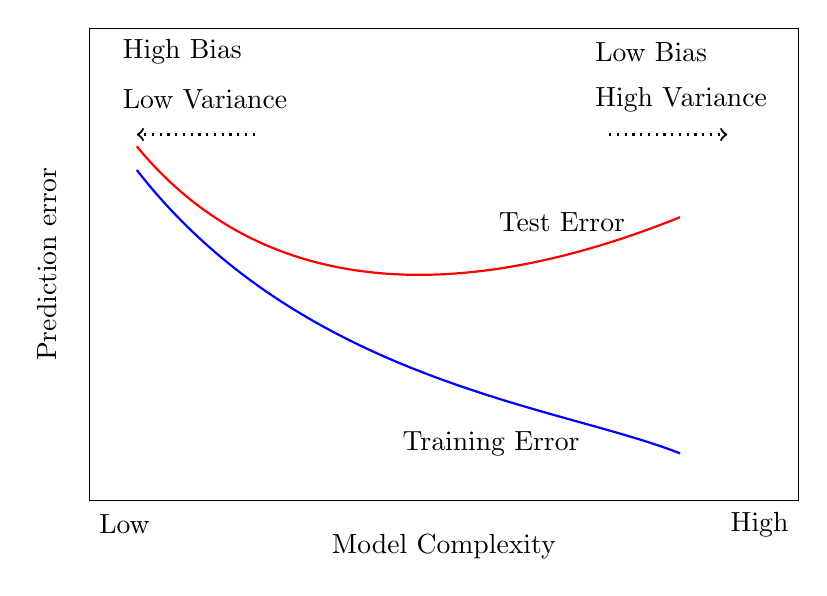
\begin{tikzpicture}[scale=3]
        \draw[] (0,0) rectangle (3,2);
        \draw[red, thick] (0.2,1.5) .. controls (0.9,0.65) and (2,1) .. (2.5,1.2);
        \draw[blue, thick] (0.2,1.4) .. controls (0.9,0.5) and (2,0.4) .. (2.5,0.2);
        \draw[->, dotted, thick] (0.7,1.55)--(0.2,1.55);
        \draw[->, dotted, thick] (2.2,1.55)--(2.7,1.55);
        \node[anchor=south] at (2,1.1) {Test Error};
        \node[anchor=south] at (1.7,0.15) {Training Error};
        \node[anchor=west] at (2.1,1.9) {Low Bias};
        \node[anchor=west] at (2.1,1.7) {High Variance};
        \node[anchor=west] at (0.1,1.9) {High Bias};
        \node[anchor=west] at (0.1,1.7) {Low Variance};
        \node[anchor=west] at (0,-0.1) {Low};
        \node[anchor=east] at (3,-0.1) {High};
        \node[anchor=south, rotate= 90] at (-0.1,1) {Prediction error};
        \node[anchor=north] at (1.5,-0.1) {Model Complexity};
    \end{tikzpicture}
    \fi
    \caption[Model complexity vs prediction error]{Illustration of how an increase in model complexity does not necessarily mean a lower prediction error when tested on new data. Thus, this can also be seen as an illustration of the Bias-Variance trade-off in model selection.}
    \label{fig:model_complexity}
\end{figure}

In search for the optimal model with the right complexity, one can constrain the hypothesis space to some extent.\footnote{The full hypothesis space is the space of all models ${f:\mathbb{R}^M \to \mathbb{R}}$, where $M$ is the number of features in the feature vector} For the sake of example, one could assume a linear relationship between the attributes, i.e., assuming that a target $y$ can be modelled as linear combinations of the features with weights $\bsw$ \eqref{lin_relation} 
\begin{equation}\label{eq:lin_relation}
    f\qty(\xxx,\bsw)  =  \xxx^{\top} \bsw  +w_0 
\end{equation} 

and thereby constrain the hypothesis space to the space of linear models.
In the supervised learning regime illustrated in \figref{supervised_learning}, we try to model inputs $\xxx$ to given outputs $y$, 
\begin{align}\label{eq:supervised_modelling}
    y&=f\qty(\xxx,\bsw) + \varepsilon
\end{align}
Where the modelling function $f\qty(\xxx,\bsw)$ is a function of the fixed feature vector $\xxx$ where the weights of the individual attributes are given as $\bsw$. The $\varepsilon$ parameter represents an unknown error term due to noise. The learning part of these supervised methods is then to optimize the weights based on the data set $\mathcal{D}$ in order to predict new observations accurately. Due to the results of this project being produced by a linear regression model, further elaboration of the linear regression model is considered appropriate.

\subsubsection{The Linear Regression Model}
The linear model assumes the targets $\yyy$ can be modelled as a linear function of the feature vector $\xxx$. Assuming that the data has been standardized (centered), the linear model are given as 
\begin{equation}\label{eq:lin_standard}
    f\qty(\xxx,\bsw) = \xxx^{\top} \bsw
\end{equation}

When trying to fit a proper model according to the machine learning method described in \secref{mlmethod}, one will then attempt to optimize the weights by minimizing a dissimilarity measure. The dissimilarity measure/error function used for the linear regression model is the residual sum of squares\index{Residual Sum of Squares} and the optimization \index{Optimization}problem is given as, 
\begin{equation}
    \bsw^* = \argmin_{\bsw} \curlyb{E\qty(\bsw)} = \argmin_{\bsw} \curlyb{\sum_{i=1}^{N} \qty(\hat{y}_i-\xxx^{\top} \bsw)^2}
\end{equation}
and with analysis, $\bsw^*$ can be found in terms of the data matrix $\XXX$ and the targets $\yyy$ as
\begin{equation}\label{eq:non_penalized_lin_model}
    \bsw^* = \qty( \XXXtilde^{\top} \XXXtilde )^{-1} \XXXtilde^{\top} \yyy
\end{equation}
Derivations of these results can be found in \appref{derivations}. 

\subsection{Penalization of the linear regression model}\label{sec:linmodel}
\index{Ordinary Least Squares}\index{Residual Sum of Squares}\index{Penalization}
As earlier stated, the linear regression model assumes that the targets can be predicted by linear combinations of the attributes of $\xxx$, which takes the form of \eqref{lin_relation}.   
The \emph{Ordinary Least Squares} (OLS) method is a linear regression model utilizing that the optimization of the weights is done using the \emph{residual sum of squares} (RSS) as the error function. The optimal weights $\bsw^*$ is then obtained by minimizing the residual sum of squares with respect to the weight vector\footnote{Again assuming that the data is centered, so that the bias weight $w_0$ can be neglected.}, $\bsw$, \begin{equation}\label{eq:ordinary_least_squares}
    \begin{split}
    \bsw^{*} = \argmin_{\bsw} \left\{\mathrm{RSS}\qty(\bsw) \right\} &= \argmin_{\bsw} \left\{ \sum_{i=1}^{N} \qty(\hat{y}_i - f\qty(\xxx_i))^2 \right\}\\
    &=\argmin_{\bsw} \left\{ \sum_{i=1}^{N} \qty( \hat{y}_i - \xxx^{\top} \bsw)^2 \right\}
    \end{split}
\end{equation}
A nice property of the linear regression is that it can be arbitrarily complex and take non-linear relations into account by introducing feature transformations, described in \secref{dataprep}, i.e., one can account for non-linear relationships by introducing feature transformations such as squaring the initial attributes. These feature transformations can exploit other proportionalities between the feature vectors and targets, but they increase the model complexity \index{Model Complexity} as well, which might result in overfitting the data. Thus, the optimization problem can be restated as finding the perfect balance between bias and variance, as illustrated in \figref{model_complexity}. The \emph{bias-variance trade-off} can be taken into consideration by penalizing the error function. Examples of such penalizations are the Lasso and the Ridge regressions. The benefits of applying coefficient shrinkage like Lasso\index{Lasso} and Ridge \index{Ridge Regression}is not just the consideration of the bias-variance trade-off\index{Bias-Variance Trade-off}, but both regression\index{Regression} types also increase the interpretability of a given model due to the fact that they allow weights for irrelevant attributes to shrink towards zero.

\subsubsection{Least Absolute Shrinkage and Selection Operator (Lasso)}
Like OLS, Lasso optimizes the residual sum of squares with respect to the weights, but adds the constraint that the sum of absolute values of weights should be less or equal to some shrinkage parameter $s$ which has to be chosen appropriately. Thus the formal formulation for the Lasso method is as \eqref{ordinary_least_squares} under the extra constraint that,
\begin{equation}\label{eq:lasso_shrinkage_constraint}
\sum_{j=1}^{M} \left| w_j \right| \leq s
\end{equation}
If the $s$ parameter is less than the full OLS estimate, this penalization will cause the weights of less important attributes to shrink until some truncate at $w_k=0$ is reached in order to fulfill \eqref{lasso_shrinkage_constraint}. This is equivalent to the problem of minimizing: 
\begin{equation}\label{eq:lasso_prob}
    \bsw^{*} = \argmin_{\bsw} \left\{ \sum_{i=1}^{N} \qty(y_i -\bsw^{\top} \xxx_i)^2 + \lambda \sum_{j=1}^{M} \left| w_j \right| \right\}
\end{equation}
where the value of $\lambda$ indicates the amount of shrinkage, i.e., a bigger value of $\lambda$ implies more shrinkage and thus more bias added to the model and vice versa with smaller values of $\lambda$ which means that less bias is introduced.\footnote{$\lambda$ is generally referred to as the regularization strength and usually takes on values in the range of $10^{-5}$ to 1.} Regularization is thus a method of substantially reducing the variance of a model without introducing too much bias if $\lambda$ is chosen wisely. The concepts of regularization arises naturally from probability theory by acknowledging that the prior probability distribution of the weights, $p\qty(\bsw)$ is not supposed to be ignored/assumed uniform in the derivation of the OLS.\footnote{However, proof of this statement will not be included in this project, but can be found in a lot of literature, e.g. \citep{allhailkingMorten}}


\paragraph{The difference between Lasso and Ridge} lies in the \Lnorm{p} used to penalize the residual sum of squares. Whereas Lasso uses the \Lnorm{1}, Ridge regression regularizes using a \Lnorm{2}.\footnote{This results in the solutions to the optimization problem for Lasso being non-linear in $y$ while the solutions to the Ridge optimization problem is linear in $y$} To understand the difference between the two penalization types, the geometry of Lasso and Ridge will be studied briefly using the OLS criterion which is equivalent to the quadratic function,
\begin{align}
    \qty(\bsw - \bsw^0)^{\top} \XXXtilde^{\top} \XXXtilde (\bsw - \bsw^0)+C
\end{align}
where $\bsw^0$ is the full OLS estimate without shrinkage and $C$ is a constant. In \figref{lassovsridge}, the contours of this quadratic function are outlined as well as the constraint regions for the Lasso ($L_1$-norm) and Ridge ($L_2$-norm) respectively. In the two dimensional case of \figref{lassovsridge} it is seen that the contours can hit the tip of the constraint region in the Lasso case. If this happens, one of the two weights will become equal to zero. In the Ridge case, the weights can only become $\approx 0$. This two dimensional example can easily be expanded and hence the Lasso allows for sparse solutions in regards to the number of features. 

The decision about whether to apply a Lasso- or Ridge penalization, as usual, requires the machine learning practitioner to think about the data set in hand. According to the results found by \citep{Tibshirani94regressionshrinkage}, the Ridge penalization is performing better than Lasso when the target values can be predicted by many small effects, whereas Lasso performs best when there is a small to moderate number of features that contribute to predict the targets, as \figref{lassovsridge} suggests as well.

In this project, we would like to create an as low dimensional feature vector as possible, i.e. look for the smallest set of features being able to predict the targets of our model fairly accurately. Hence, the \Lnorm{1} seems like the preferable choice of regularization. However, since we would like to find the smallest possible set of features able to predict our targets, it is worth considering sequential feature selection.\index{Sequential Feature Selection}\index{Forward Selection}

\paragraph{Forward selection} iterates through the features one by one and adds the feature with the lowest test error $E_{\mathrm{test}}$ to the optimal set of features. It then tries to add another feature to the feature vector by searching for candidates that can lower the error compared to the single feature. If multiple features can lower $E_{\mathrm{test}}$, the one that results in the largest decrease in test error will be chosen. The algorithm then continues until the test error cannot be decreased by addition of another feature. According to \citep{Tibshirani94regressionshrinkage}, this method is preferable when there is a small amount of large effects, i.e. a small amount of highly important features.
%%%%%%%%%%%%%%%%%%%%%%%%%%%%%%%%%%%
%   Lasso vs Ridge penalty plot   %
%%%%%%%%%%%%%%%%%%%%%%%%%%%%%%%%%%%

\begin{figure}[t]
    \centering
    %First pictures
   
    \begin{subfigure}[b]{0.45\textwidth}
    \iffigure
        \begin{tikzpicture}
            \begin{axis}[no markers,xlabel=$\hat{w}_1$, 
                ylabel=$\hat{w}_2$,
                ticks=none,
                axis x line=center,
                axis y line=center,
                ymin=-1.1,
                xmin=-1.1,
                xmax=2,
                ymax=3,
                axis equal]
                \addplot+[fill=softblue, color=softblue, opacity=0.5] coordinates
                {(-1,0) (0,1) (1,0) (0,-1)}--cycle;
                \draw[red] (1,2) ellipse [x radius=0.4, y radius=0.2, rotate=45];
                \draw[red] (1,2) ellipse [x radius=0.6, y radius=0.3, rotate=45];
                \draw[red] (1,2) ellipse [x radius=1, y radius=0.5, rotate=45];
                \draw[red] (1,2) ellipse [x radius=1.4, y radius=0.7, rotate=45];
                \node[] at (1,2) {$\hat{w}$};
            \end{axis}
            %
        \end{tikzpicture}
        \fi
    \end{subfigure}
    \quad
    %Second picture
    \begin{subfigure}[b]{0.45\textwidth}
    \iffigure
        \begin{tikzpicture}
            \begin{axis}[no markers,xlabel=$\hat{w}_1$, 
                ylabel=$\hat{w}_2$,
                ticks=none,
                axis x line=center,
                axis y line=center,
                ymin=-1.1,
                xmin=-1.1,
                xmax=2,
                ymax=3,
                axis equal]
                \filldraw[draw=softblue, fill=softblue, opacity=0.5] (0,0) circle (1);
                \draw[red] (1,2) ellipse [x radius=0.4, y radius=0.2, rotate=45];
                \draw[red] (1,2) ellipse [x radius=0.6, y radius=0.3, rotate=45];
                \draw[red] (1,2) ellipse [x radius=1, y radius=0.5, rotate=45];
                \draw[red] (1,2) ellipse [x radius=1.3, y radius=0.65, rotate=45];
                \node[] at (1,2) {$\hat{w}$};
            \end{axis}
        \end{tikzpicture}
        \fi
    \end{subfigure}
    
    \caption[Lasso versus Ridge Shrinkage]{Illustration of how the Least Absolute Shrinkage and Selection Operator (Lasso) is able to set some weights of features to 0 (using the \Lnorm{1}) whereas Ridge regression only allow specific feature weights to be $\approx$ 0 but $\neq$ 0 (using the \Lnorm{2}). The figure on the left shows a \Lnorm{1} and on the right a \Lnorm{2}.}
    \label{fig:lassovsridge}
\end{figure}

%%%%%%%%%%%%%%%%%%%%%%%%%%%%%%%%%%%%

\seclab{Model selection and performance Evaluation}{mspe}\index{Model Selection}\index{Performance Evaluation}
When performing model selection, one should assess the optimal model as the model which generalizes best to unseen data, i.e., to search for the model that will minimize the test error curve in \figref{model_complexity}. But the test error is specific to a given test, hence, to get the true prediction error, one would like to test the model on as much unseen data as possible and ideally, an infinite amount of data. The generalization error, which is an idealized quantity, is introduced as the error the model would have, had it been tested on an infinite amount of test data $\notin$ $\mathcal{D}_{\mathrm{train}}$.

\subsection{Cross-validation}\label{sec:crossvalidation}\index{Cross-Validation}

\begin{figure}[ht]
    \centering
    \iffigure
    \begin{tikzpicture}
    
        %First line
        \filldraw[draw=softblue, fill=softblue] (0,3.5) rectangle (12,4.5);
        % third line
        \filldraw[draw=softblue, fill=softblue] (0,2) rectangle (12,3);
        \filldraw[draw=softgrey, fill=softgrey] (0,2) rectangle (4,3);
        %fourth line
        \filldraw[draw=softblue, fill=softblue] (0,0.5) rectangle (12,1.5);
        \filldraw[draw=softgrey, fill=softgrey] (4,0.5) rectangle (8,1.5);
        %fith line
        \filldraw[draw=softblue, fill=softblue] (0,-1) rectangle (12,0);
        \filldraw[draw=softgrey, fill=softgrey] (8,-1) rectangle (12,0);
        %Legend
        \node[] at (6,4) {$N$};
        
        \node[] at (2,2.5) {$\dfrac{1}{3}N$ };
        \node[] at (8,2.5) {$\dfrac{2}{3}N$ };
        
        \filldraw[draw=softblue, fill=softblue] (0,5) rectangle (0.5,5.5);
        \node[anchor=west] at (0.5,5.25) {Training data};
        
        \filldraw[draw=softgrey, fill=softgrey] (9.5,5) rectangle (10,5.5);
        \node[anchor=west] at (10,5.25) {Test data};
        
        
    \end{tikzpicture}
    \fi
    \caption[Cross-validation illustration]{Visual example of $K$-fold CV; Here seen a 3-fold validation where the data set is split into subsets, $\mathcal{D} = \mathcal{D}_1 \cup \mathcal{D}_2 \cup \mathcal{D}_3 $. For each subset, the model is trained on 2/3 and tested on 1/3 of the total $N$ observations.}
    \label{fig:kfold}
\end{figure}


\emph{Cross-validation} (CV) is a technique which beautifully takes into account, that when finding the optimal model for a problem, one must not test the model on the data used for training. The idea behind CV, is to create as much test and training data using only the data set itself. There are three major types of cross-validation, \emph{Hold-Out} CV, \emph{K}-fold CV and \emph{Leave-one-out} Cross-validation\citep{allhailkingMorten}. In this project, \emph{K}-fold has been used exclusively. Both for model selection and estimating the generalization error of the optimal model. When performing $K$-fold CV, the data set is split into $K$ subsets, $\mathcal{D} = \mathcal{D}_1 \cup  ... \cup \mathcal{D}_k \cup ... \cup \mathcal{D}_K$. Hence, $K$-fold CV allows one to test the models on the entire data set.

In $K$-fold CV, the idealized generalization error \index{Generalization Error} is approximated as:
\begin{equation}\label{eq:gen_error}
    \EM{gen} \approx \sum_{k=1}^K \dfrac{N_{k}^{\mathrm{test}}}{N}   E_{\mathcal{M},k}^{\mathrm{test}}
\end{equation}
where $N_k^{\mathrm{test}}$ is the number of observations for testing in fold number $k$, and $\EMss{,k}{test}$ is given as
\begin{equation}
    \EMss{,k}{test} = \dfrac{1}{N_{k}^{\mathrm{test}}} \sum_{i \in \Dtest} d\qty(y_i,\FM{\xxx_i,\bsw})
\end{equation}
The appropriate dissimilarity measure varies from task to task, but recall that in the case of regression, one uses the RSS. An illustrative example of how the data is split for a $3$-fold CV is seen in \figref{kfold}.

CV can be used for both model selection and estimation of the generalization error. Two-layer CV is a way of doing both and thus getting an unbiased estimate of the generalization error. This is done for every model created in the code phase of this project. Therefore the procedure is outlined in pseudo-code in Algorithm \ref{algo:tlcv}\footnote{The idea of outlining the Algorithm in pseudo-code is due to \citep{allhailkingMorten}}.
\begin{algorithm}
\caption{$K$-Fold Cross-Validation for Model selection and $\EM{gen}$ estimation}

\begin{algorithmic}[0]

\Require{$K_1$ folds in outer loop for estimation of the generalization error}
\Require{$K_2$ folds in inner loop for model selection}
\Require{$S$ models to cross-validate: $\mathcal{M}_1 , ... , \mathcal{M}_S$}
\Ensure{$\hat{E}_{\mathcal{M}*}^{\mathrm{gen}}$}

\For{$i =1,...,K_1$}
    \State{\emph{Outer CV loop. The data set, $\calD$ is split into $K_1$ folds} }
    \State{The $i$'th split of $\calD$ is $\calD_{i}^{\mathrm{par}},\calD_{i}^{\mathrm{test}}$}
    \For{$j=1,...,K_2$}
        \State{\emph{Inner CV loop doing $K_2$ splits for model selection testing $S$ models}}
        \State{The $j$'th split of $\calD_i^{\mathrm{par}}$ is $\calDss{j}{train},\calDss{j}{val}$} 
        \For{$s=1,...,S$}
            \State{Train $\mathcal{M}_s$ on $\calDss{j}{train}$ }
            \State{Let $\EMss{_{s,j}}{val}$ be the \emph{validation error} of the model $\mathcal{M}_s$ when it is \emph{tested} on $\calDss{j}{val}$}
        \EndFor
    \EndFor    
    \State{For each $s$ compute $\hat{E}_s^{\mathrm{gen}}= \sum_{j=1}^{K_2} \frac{\abs{\calDss{j}{val}}}{\calDss{i}{par}} \EMss{_s,j}{val}$ }
    \State{Select the optimal model $\mathcal{M}^*$ = $\mathcal{M}_{s^*}$ where $s^* = \argmin_s \hat{E}_s^{\mathrm{gen}}$}
    \State{Train $\mathcal{M}^*$ on $\calDss{i}{par}$}
    \State{Let $E_i^{\mathrm{test}}$ be the \emph{test error} of the model $\mathcal{M}^*$ when it is tested on $\calDss{i}{test}$}
\EndFor
\State{Compute the estimate of the generalization error: $\hat{E}^{\mathrm{gen}} = \sum_{i}^{K_1} \frac{\abs{\calDss{i}{test}}}{N} E_i^{\mathrm{test}}$}
\end{algorithmic}
\label{algo:tlcv}
\end{algorithm}








\chapter{Machine learning in physics}\label{chap:ml_in_physics}
\thispagestyle{empty}
%%%%%%%%%%%%%%%%%%%%%%%%%%%%%%%%%%%%%%%%%%%%%%%%%%%%%
%   Chapter 2: OUTLINE                              %
%%%%%%%%%%%%%%%%%%%%%%%%%%%%%%%%%%%%%%%%%%%%%%%%%%%%%
Quantum simulation methods like density functional theory and quantum Monte Carlo simulations have facilitated accurate calculations of quantum systems. The amount of quantum simulations performed on a daily basis is immense, but these methods have their restrictions. The time consumption of a DFT simulation increases significantly with the amount of atoms, i.e. $T\sim N^{\alpha}$ with $\alpha \approx 2-3$ and $N$ the number of atoms \citep{KohnNobelLecture}. Thus, if one could predict different material properties more efficiently it would be beneficial to the field of material sciences. The tools of machine learning bring possibilities of doing just that. For example, the situation where a group has done extensive research with quantum simulations on a system of interest. The data achieved by performing these computationally costly simulations can with proper ML methods promote knowledge about the systems of interest as illustrated in \figref{mlandquant}. The figure illustrates how ML can contribute to material sciences by learning from quantum simulated data and additional knowledge about the systems. 
\begin{figure}[ht]
    \centering
    %\iffigure
        \begin{tikzpicture}

        \filldraw[fill=softblue, draw=softblue,ultra thick, rounded corners=15pt, opacity=0.5 ] (-3.5,0.5) rectangle (3.5,2);
        \filldraw[fill=softblue, draw=softblue,ultra thick, rounded corners=15pt, opacity=0.5] (-3.5,-2) rectangle (3.5,-0.5);
        \filldraw[fill=softblue, draw=softblue,ultra thick, rounded corners=15pt, opacity=0.5] (-3.5,-4.5) rectangle (3.5,-3);
        \draw[ultra thick,->, rounded corners=15pt] (3.5,-3.75)--(4.5,-3.75)--(4.5,1.25)--(3.5,1.25);
        \draw[->, ultra thick] (0,0.5)--(0,-0.5);
        \draw[->, ultra thick] (0,-2)--(0,-3);
        
        \node[] at (0,1.25) {Systems of interest (SOI)};
        
        \node[] at (0, -1.25) {Data to be used for ML};
        \node[] at (0,-3.75) {ML model for predictions, $\hat{y}$};
        \node[anchor=south east] at (0,-0.5) {QM computation};
        \node[anchor=south east] at (0,-3) {ML algorithm};
        \node[anchor=west] at (4.5,-1.25) {\rotatebox[origin=c]{270}{Supplementary understanding of SOI}};
    \end{tikzpicture}
    %\fi
    \caption[Machine learning and Quantum Computations]{Illustration of how quantum theory and machine learning can help each other in predicting properties of materials. Machine learning can help speed up the computations by predicting and validating the best candidates as the computation provides raw data for the machine learning model to train on. }
    \label{fig:mlandquant}
\end{figure}
The thoughts about ML and material sciences has consequently brought a lot of attention to the subject and therefore a quick review of the already implemented methods is considered convenient.

\seclab{Implemented ML methods in materials science}{donesofar}

 Several approaches to utilize machine learning algorithms in material science and physics have been made in recent times \citep{mueller_kussesne,criticalrole_descriptor,frameworkforML}. The approaches include predictions of phase diagrams \citep{phasediagram,phase2diagrams}, predictions of various material properties based on data from quantum mechanical computations \citep{rupp,Pilania2013}, interatomic potentials development \citep{hansen2015a,huan2015a, bartok2010a, behler2011a, behler2007a}, predictions of crystal structures  \citep{woodley2008a,madoxx1988,fischer2006a}, discovering and developing density functionals \citep{behler2011ANN}, modelling of crystal lattices \citep{mueller2009a, mueller2012a, seko2009a} along with behavior and processing of complex materials \citep{metzbower2001a, bucholz2012a}.
While some of these are somewhat out of the scope of this project they resemble what can be achieved using machine learning as an asset to established methods in materials science and engineering. An approach related to the procedure of this project was performed by \emph{Rupp et al.} \citep{rupp} who used a ridge regression with a Gaussian Kernel to predict accurate molecular atomization energies. Their data set, which was calculated with\index{Density Functional Theory} (DFT), contained more than 7000 organic molecules, each consisting of up to 7 atoms and they achieved a \emph{Root Mean Squared Error} (RMSE) of $\approx$ 1.3 eV per molecule and a \emph{Mean Absolute Arror} of $\approx$ 0.65 eV per molecule for the machine learning method. 
Another study closely related to this project \citep{criticalrole_descriptor} investigates how to use the Lasso \index{Lasso} method for feature selection in order to predict the difference in energies for two different structures of binary compounds. The purpose of their studies was to outline the critical role of using a suitable feature vector and investigates if a low-dimensional representation of the feature vector would be able to predict the target values. The data set used by \emph{Ghiringhelli} and \emph{Scheffler} consists of 82 binary octet materials, $N=82$, with the target values $\yyy$ = \emph{"The energy differences between the rock salt crystal structure and the zinc blende or wurtzite structures"}. We will strive to do something similar in this project, however, being able to find as low-dimensional feature vectors is unlikely, due our model being more complex as non-octet sets are considered. 
Among all the different ways to implement machine learning in materials science, using the Lasso can serve as a suitable method, since one can create arbitrarily complex feature transformations in accordance to \secref{dataprep} and then penalize the model to reduce complexity to the right amount by using CV for model selection. By doing so, one can introduce the right amount of bias and variance to create a well-generalizing model which keeps its interpretability intact.

\seclab{Predicting the difference in heat of formation between four crystal structures}{main_model}\index{Heat of Formation}\index{Crystal Structures}
%We are living in a time where a lot of research in materials sciences focus on exploration of materials with specific properties for specific purposes. For example, the search for possible materials to be utilized in photovoltaic solar cells. In such a search, it is common to start with a screening phase where a lot of potential candidates are discarded. Even though computer science has evolved a lot in recent years and we can run computationally expensive molecular simulations, methods like DFT and Quantum Clustering can be considered inefficient in such screening processes as they are computationally too costly for the purpose.
The hope of this project is to create a machine learning model able to contribute to the current goals of materials science. Ideally, through the modelling of this project, we can create a universal set of features being able to accurately predict which of the considered crystal structures is the most stable. By doing so, one could reduce the amount of more advanced quantum simulations significantly. 
\subsection{The crystal structures used in the project}
\begin{table}[ht]
    \centering
    \begin{tabular}{cccccc}
    \toprule
    Kind of atom  & \multicolumn{4}{c}{Atom} \\\midrule
    \multirow{11}{*}{\textbf{A}} 
        & Li & Be & B & Na  \\
        & Mg & Al & Si & K  \\
        & Ca & Sc & Ti & Zn \\
        & Ga & Ge & As & Rb  \\ 
        & Sr & Y & Zr & Nb  \\
        & Mo & Ru & Rh & Pd  \\
        & Ag & Cd & In & Sn  \\
        & Sb & Te & Cs & Ba  \\
        & La & Hf & Ta & Re  \\
        & Os & Ir & Pt & Au  \\\midrule
    \multirow{4}{*}{\textbf{B}}    
        & B & C & N & O   \\
        & F & Si & P & S   \\
        & Cl & Ge & As & Se   \\
        & Br & Sb & Te & I   \\\bottomrule
    \end{tabular}
    \caption[The different A and B atoms used]{Identification of the different A and B atoms used to construct the dimers. As seen, there are $44 \times 16 = 704$ different combinations, given us 704 rows of data to be used for machine learning.}
    \label{tab:ABcompounds}
\end{table}

This project has examined four different data sets. Each data set containing the heat of formation, $\Delta H$ of AB compounds calculated with DFT for different crystal structures. The four different structures examined are \emph{Rock Salt} (Rs), \emph{Nickel Arsenide} (NiAs), \emph{Zinc Blende} (Zb) and \emph{Wurtzite} (Wz) and unit cells for each can be seen on \figsref{rs}{nias}{zb}{wz}. In each of the four data sets, there are 44 different A atoms and 16 different B atoms and the data sets contain every combination of A and B. This gives a total of $N = 44 \times 16 = 704$ observations; the different A and B atoms are outlined in \tabref{ABcompounds}.

To get the most data out the model, a machine, that via. a reference structure is able to predict the energy differences between all of the four crystal structures using a multi-target regression, is to prefer. If such a model can be constructed, one would be able get a lot of information out of a a single feature vector $\xxx_i$. 

The target values for the different models that will be constructed is thus, 
\begin{align}
  \hat{y} = \Delta H_{cs \neq r} - \Delta H_{r}  
\end{align}
i.e., if the reference structure as an example is Rock Salt, then $\Delta H_{r} = \Delta H_{\mathrm{Rs}}$ and $\Delta H_{cs \neq r} = \curlyb{\Delta H_{\mathrm{NiAs}},\Delta H_{\mathrm{Zb}},\Delta H_{\mathrm{Wz}}}$
\begin{figure}
    \begin{subfigure}[b]{0.45\textwidth}
    \centering
    \iffigure
    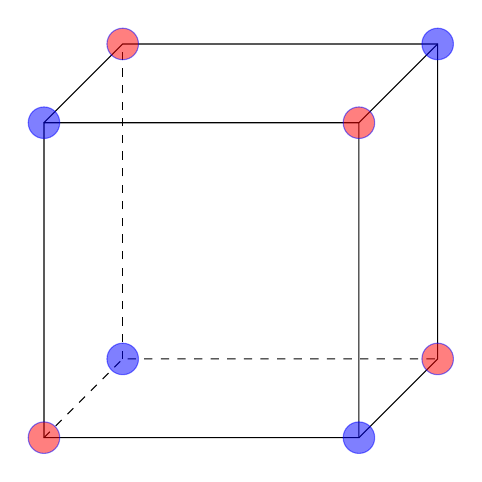
\begin{tikzpicture}
    %Firkant
        \draw[] (0,0) rectangle (4,4)--(5,5);
        \draw[] (0,4)--(1,5)--(5,5)--(5,1)--(4,0);
        \draw[dashed] (0,0)--(1,1)--(5,1) ;
        \draw[dashed] (1,1)--(1,5);

    %Atomer    
        \filldraw[fill=red, draw=blue,opacity=0.5] (0,0) circle (0.2);
        \filldraw[fill=blue, draw=blue,opacity=0.5] (4,0) circle (0.2);
        \filldraw[fill=blue, draw=blue,opacity=0.5] (0,4) circle (0.2);
        \filldraw[fill=red, draw=blue,opacity=0.5] (4,4) circle (0.2);
        \filldraw[fill=blue, draw=blue,opacity=0.5] (1,1) circle (0.2);
        \filldraw[fill=red, draw=blue,opacity=0.5] (5,1) circle (0.2);
        \filldraw[fill=red, draw=blue,opacity=0.5] (1,5) circle (0.2);
        \filldraw[fill=blue, draw=blue,opacity=0.5] (5,5) circle (0.2);
        
        %
    \end{tikzpicture}
    \fi
    \caption{Crystal Structure of Rock Salt (RS). }
    \label{fig:rs}
    \end{subfigure}
    %
    \quad
    %
    \begin{subfigure}[b]{0.45\textwidth}
    \centering
    \iffigure
    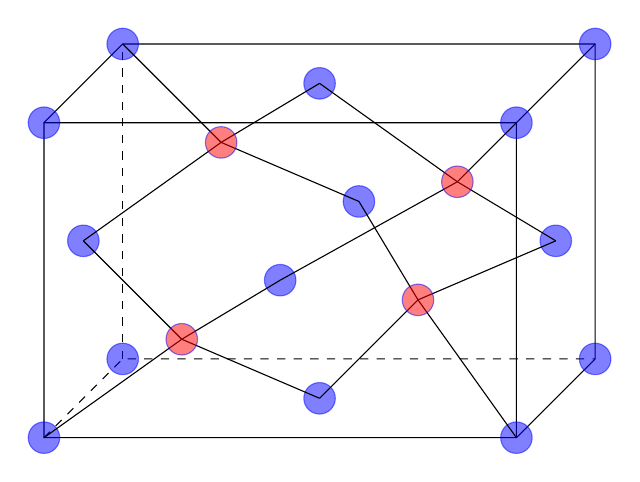
\begin{tikzpicture}
    %Firkant
        \draw[] (0,0) rectangle (6,4)--(7,5);
        \draw[] (0,4)--(1,5)--(7,5)--(7,1)--(6,0);
        \draw[dashed] (0,0)--(1,1)--(7,1) ;
        \draw[dashed] (1,1)--(1,5);

    %Atomer    
        \filldraw[fill=blue, draw=blue,opacity=0.5] (0,0) circle (0.2);
        \filldraw[fill=blue, draw=blue,opacity=0.5] (6,0) circle (0.2);
        \filldraw[fill=blue, draw=blue,opacity=0.5] (0,4) circle (0.2);
        \filldraw[fill=blue, draw=blue,opacity=0.5] (6,4) circle (0.2);
        \filldraw[fill=blue, draw=blue,opacity=0.5] (1,1) circle (0.2);
        \filldraw[fill=blue, draw=blue,opacity=0.5] (7,1) circle (0.2);
        \filldraw[fill=blue, draw=blue,opacity=0.5] (1,5) circle (0.2);
        \filldraw[fill=blue, draw=blue,opacity=0.5] (7,5) circle (0.2);
        %
        \filldraw[fill=blue, draw=blue,opacity=0.5] (0.5,2.5) circle (0.2);
        \filldraw[fill=blue, draw=blue,opacity=0.5] (6.5,2.5) circle (0.2);
        \filldraw[fill=blue, draw=blue,opacity=0.5] (3,2) circle (0.2);
        \filldraw[fill=blue, draw=blue,opacity=0.5] (4,3) circle (0.2);
        \filldraw[fill=blue, draw=blue,opacity=0.5] (3.5,0.5) circle (0.2);
        \filldraw[fill=blue, draw=blue,opacity=0.5] (3.5,4.5) circle (0.2);
        %
        \draw[thin] (0,0)--(1.75,1.25);
        \draw[thin] (0.5,2.5)--(1.75,1.25);
        \draw[thin] (3,2)--(1.75,1.25);
        \draw[thin] (3.5,0.5)--(1.75,1.25);
        
        \draw[thin] (3.5,0.5)--(4.75,1.75);
        \draw[thin] (4,3)--(4.75,1.75);
        \draw[thin] (6,0)--(4.75,1.75);
        \draw[thin] (6.5,2.5)--(4.75,1.75);
        
        \draw[thin] (1,5)--(2.25,3.75);
        \draw[thin] (0.5,2.5)--(2.25,3.75);
        \draw[thin] (3.5,4.5)--(2.25,3.75);
        \draw[thin] (4,3)--(2.25,3.75);
        
        \draw[thin] (3,2)--(5.25,3.25);
        \draw[thin] (3.5,4.5)--(5.25,3.25);
        \draw[thin] (6,4)--(5.25,3.25);
        \draw[thin] (6.5,2.5)--(5.25,3.25);
        %
        \filldraw[fill=red, draw=blue,opacity=0.5] (2.25,3.75) circle (0.2);
        \filldraw[fill=red, draw=blue,opacity=0.5] (1.75,1.25) circle (0.2);
        \filldraw[fill=red, draw=blue,opacity=0.5] (5.25,3.25) circle (0.2);
        \filldraw[fill=red, draw=blue,opacity=0.5] (4.75,1.75) circle (0.2);
    \end{tikzpicture}
    \fi
    \caption{Crystal structure of Zinc blende (ZB).}
    \label{fig:zb}
    \end{subfigure}
    \\
    \begin{subfigure}[b]{0.45\textwidth}
    \centering
    \iffigure
    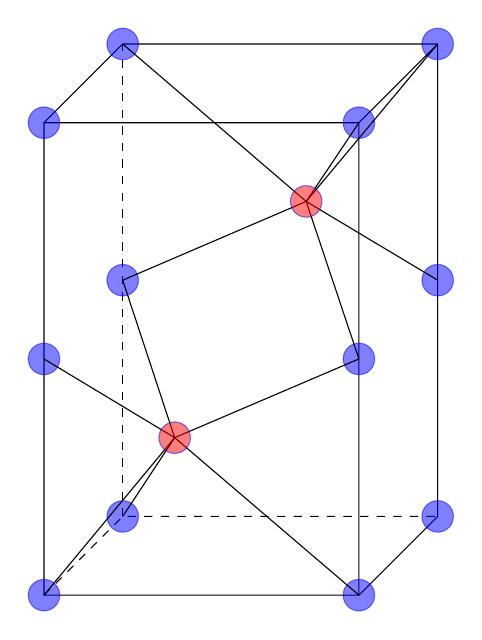
\begin{tikzpicture}
    %Firkant
        \draw[] (0,0) rectangle (4,6)--(5,7);
        \draw[] (0,6)--(1,7)--(5,7)--(5,1)--(4,0);
        \draw[dashed] (0,0)--(1,1)--(5,1) ;
        \draw[dashed] (1,1)--(1,7);
   \iffalse
    %Koordinatsystem
        \draw[thick,->] (-3,0)--(-1,0);
        \draw[thick,->] (-3,0)--(-2.5,0.5);
        \draw[thick,->] (-3,0)--(-3,2);
        \node[anchor=west] at (-1,0) {$x$};
        \node[anchor=west] at (-2.5,0.5) {$y$};
        \node[anchor=west] at (-3,2) {$z$};
    \fi
    %Atomer    
        \filldraw[fill=blue, draw=blue,opacity=0.5] (0,0) circle (0.2);
        \filldraw[fill=blue, draw=blue,opacity=0.5] (4,0) circle (0.2);
        \filldraw[fill=blue, draw=blue,opacity=0.5] (0,3) circle (0.2);
        \filldraw[fill=blue, draw=blue,opacity=0.5] (4,3) circle (0.2);
        \filldraw[fill=blue, draw=blue,opacity=0.5] (1,1) circle (0.2);
        \filldraw[fill=blue, draw=blue,opacity=0.5] (5,1) circle (0.2);
        \filldraw[fill=blue, draw=blue,opacity=0.5] (1,4) circle (0.2);
        \filldraw[fill=blue, draw=blue,opacity=0.5] (5,4) circle (0.2);
        \filldraw[fill=blue, draw=blue,opacity=0.5] (1,7) circle (0.2);
        \filldraw[fill=blue, draw=blue,opacity=0.5] (4,6) circle (0.2);
        \filldraw[fill=blue, draw=blue,opacity=0.5] (5,7) circle (0.2);
        \filldraw[fill=blue, draw=blue,opacity=0.5] (0,6) circle (0.2);
        %
        \draw[thin] (0,0)--(1.66,2);
        \draw[thin] (1,1)--(1.66,2);
        \draw[thin] (0,3)--(1.66,2);
        \draw[thin] (1,4)--(1.66,2);
        \draw[thin] (4,0)--(1.66,2);
        \draw[thin] (4,3)--(1.66,2);
        
        \draw[thin] (4,3)--(3.33,5);
        \draw[thin] (5,4)--(3.33,5);
        \draw[thin] (4,6)--(3.33,5);
        \draw[thin] (5,7)--(3.33,5);
        \draw[thin] (1,7)--(3.33,5);
        \draw[thin] (1,4)--(3.33,5);
        %
        \filldraw[fill=red, draw=blue,opacity=0.5] (3.33,5) circle (0.2);
        \filldraw[fill=red, draw=blue,opacity=0.5] (1.66,2) circle (0.2);
        % 
    \end{tikzpicture}
    \fi
    \caption{Crystal structure of Nickel Arsenide (NiAs)}
    \label{fig:nias}
    \end{subfigure}
    %
    \quad
    %
    \begin{subfigure}[b]{0.45\textwidth}
    \centering
    \iffigure
    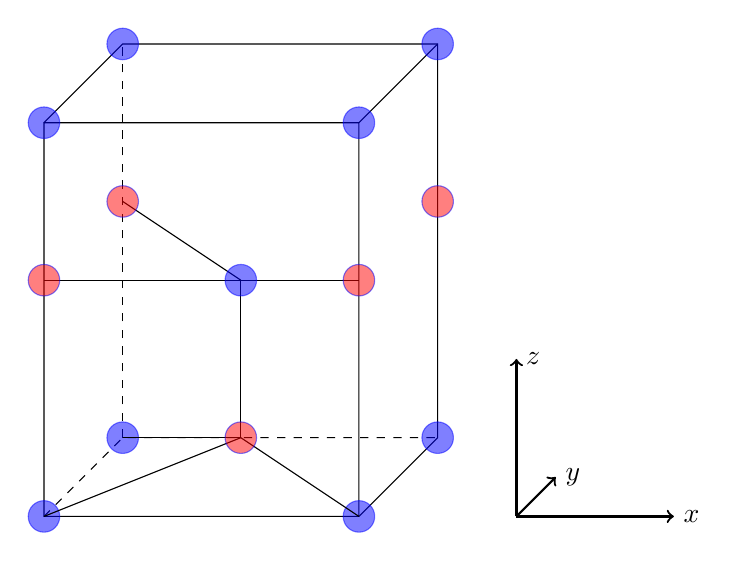
\begin{tikzpicture}
    %Firkant
        \draw[] (0,0) rectangle (4,5)--(5,6);
        \draw[] (0,5)--(1,6)--(5,6)--(5,1)--(4,0);
        \draw[dashed] (0,0)--(1,1)--(5,1) ;
        \draw[dashed] (1,1)--(1,6);

    %Atomer    
        \filldraw[fill=blue, draw=blue,opacity=0.5] (0,0) circle (0.2);
        \filldraw[fill=blue, draw=blue,opacity=0.5] (4,0) circle (0.2);
        \filldraw[fill=blue, draw=blue,opacity=0.5] (0,5) circle (0.2);
        \filldraw[fill=blue, draw=blue,opacity=0.5] (4,5) circle (0.2);
        \filldraw[fill=blue, draw=blue,opacity=0.5] (1,1) circle (0.2);
        \filldraw[fill=blue, draw=blue,opacity=0.5] (5,1) circle (0.2);
        \filldraw[fill=blue, draw=blue,opacity=0.5] (1,6) circle (0.2);
        \filldraw[fill=blue, draw=blue,opacity=0.5] (5,6) circle (0.2);
        %
        \draw[thin] (0,3)--(2.5,3);
        \draw[thin] (1,4)--(2.5,3);
        \draw[thin] (4,3)--(2.5,3);
        
        \draw[thin] (0,0)--(2.5,1);
        \draw[thin] (1,1)--(2.5,1);
        \draw[thin] (4,0)--(2.5,1);
        
        \draw[thin] (2.5,3)--(2.5,1);
        %
        \filldraw[fill=red, draw=blue,opacity=0.5] (0,3) circle (0.2);
        \filldraw[fill=red, draw=blue,opacity=0.5] (1,4) circle (0.2);
        \filldraw[fill=red, draw=blue,opacity=0.5] (4,3) circle (0.2);
        \filldraw[fill=red, draw=blue,opacity=0.5] (5,4) circle (0.2);
        %
        \filldraw[fill=blue, draw=blue,opacity=0.5] (2.5,3) circle (0.2);
        \filldraw[fill=red, draw=blue,opacity=0.5] (2.5,1) circle (0.2);
        
        
      
    %Koordinatsystem
        \draw[thick,->] (6,0)--(8,0);
        \draw[thick,->] (6,0)--(6.5,0.5);
        \draw[thick,->] (6,0)--(6,2);
        \node[anchor=west] at (8,0) {$x$};
        \node[anchor=west] at (6.5,0.5) {$y$};
        \node[anchor=west] at (6,2) {$z$};
    
    \end{tikzpicture}
    \fi
    \caption{Crystal structure of Wurtzite (WZ).}
    \label{fig:wz}
\end{subfigure}

\caption{Unitcells for the four different structures.}
\label{fig:csstruct}
\end{figure}

How the feature vector $\xxx$ for this task has been created, is described in \secref{physicsfeaturevector}.


\subsection{Creating an appropriate feature vector}\label{sec:physicsfeaturevector}
As the desirable feature vector is relatively low-dimensional and our data set containing non-octet compounds is relatively complex, it is very probable that our feature vector should include highly relevant complex attributes. Expert knowledge might come in handy and thus our strategy for creating a suitable feature vector is based on considerations from other people's work, mostly \citep{frameworkforML} and \citep{criticalrole_descriptor}. Initially, a 34-dimensional feature vector is constructed, consisting exclusively of atomic properties of the A- and B atoms and then plenty features will be constructed by feature transformations.

\subsubsection{Atomic attributes}\label{sec:atomic_att}

\pgfplotstableread[col sep=comma] {csv/basic.csv}\basic
\begin{figure}[ht]
    \centering
    \iffigure
    \begin{tikzpicture}
        \begin{axis}[boxplot/draw direction=y,
        xlabel={Attribute}, 
        ylabel={Spread},
        %xtick=data,
        xtick={1,...,17},
        xticklabels={Atom number, Group, Period, Electron negativity, Covalent radius, Atomic radius, Van der Wahls radius, Electron affinity, Ionisation energy, Average oxidation number, Difference in oxidation number, Noble gas, Number of s electrons, Number of p electrons, Number of d electrons, Pettifor radius, Atomization energy pr atom},
        x tick label style={rotate=90,anchor=east},
        enlarge x limits=-1,
        width=1\textwidth,
        height=0.5\textwidth,
        ]
        \foreach \i in {1,...,17} 
            \addplot+[boxplot]
            table[col sep=comma,y index=\i] \basic;
        \end{axis}
    \end{tikzpicture}
    \fi
    \caption[Box-plots for the initial 17 attributes of the A atom]{Boxplot of attributes for the A atom. The data is standardized as described in \secref{statmat}}
    \label{fig:boxplotA}
\end{figure}

\begin{figure}[ht]
    \centering
    \iffigure
    \begin{tikzpicture}
        \begin{axis}[boxplot/draw direction=y,
        xlabel={Attribute}, 
        ylabel={Spread},
        %xtick=data,
        xtick={1,...,17},
        xticklabels={Atom number, Group, Period, Electron negativity, Covalent radius, Atomic radius, Van der Wahls radius, Electron affinity, Ionisation energy, Average oxidation number, Difference in oxidation number, Noble gas, Number of s electrons, Number of p electrons, Number of d electrons, Pettifor radius, Atomization energy pr atom},
        x tick label style={rotate=90,anchor=east},
        enlarge x limits=-1,
        width=1\textwidth,
        height=0.5\textwidth,
        ]
        \foreach \i in {18,...,34} 
            \addplot+[boxplot]
            table[col sep=comma,y index=\i] \basic;
        \end{axis}
    \end{tikzpicture}
    \fi
    \caption[Box-plots for the initial 17 attributes of the B atom]{Boxplot of attributes for the B atom. The data is standardized as described in \secref{statmat}}
    \label{fig:boxplotB}
\end{figure}


\begin{table}[ht]
    \centering
    \begin{tabular}{|p{5cm}|c|l|}\hline
        \textbf{Attribute}                 & \textbf{Unit}  &\textbf{Type}  \\ \hline
        Atom number                 & []    &  Discrete ratio \\ \hline
        Atom group                  & []    &  Discrete ratio \\ \hline
        Atom period                 & []    &  Discrete ratio \\ \hline
        Electron negativity         & [eV]  &  Continuous ratio\\ \hline   
        Covalent radius             & [Å]   &  Continuous ratio \\ \hline
        Atom Radius                 & [Å]   &  Continuous ratio \\ \hline
        Van der Wahls radius        & [Å]   &  Continuous ratio \\ \hline
        Electron affinity           & [eV]  &  Continuous ratio \\ \hline
        Ionisation energy           & [eV]  &  Continuous ratio\\ \hline
        Average oxidation number    & []    &  Continuous ratio\\ \hline 
        Difference between largest and smallest oxidation number & [] & Continuous ratio \\ \hline
        Noble gas number      & []  & Discrete ratio  \\ \hline
        Number of s electrons & []  & Discrete ratio \\ \hline
        Number of p electrons & []  & Discrete ratio \\ \hline
        Number of d electrons & []  & Discrete ratio \\ \hline
        Pettifor radius      & [Å] & Continuous ratio \\ \hline
        Atomization energy per atom  & [eV] & Continuous ratio\\ \hline
    \end{tabular}
    \caption[Overview of the attributes used to describe an atom.]{The 17 attributes loaded from the periodic system used to generate features. The table shows units and attribute types as described in \appref{attribute_types}}
    \label{tab:att}
\end{table}

The atomic attributes in the initial feature vector are outlined in \tabref{att}, but as mentioned in \secref{dataprep}, understanding the data set is crucial. Hence, the following will elaborate on some of the initial attributes. Electron negativity describes the atoms ability to attract another electron, i.e. larger electron negativity means larger attraction. The covalent radius describes the distance an atom would have to another when forming a covalent bond. The atomic radius reflects the ionic radius, which describes the distance to the nearest atom when forming an ionic bond. Another radius to be considered is the Van der Wahls radius. The Van der Wahls radius describes the closest distance one atom can approach another in a hard sphere approximation. Electron affinity describes the cost in energy for adding another electron to the atom in its natural state. The ionization energy is the amount of energy spend to remove the most loosely bounded valence electron. As each atom can have different oxidation numbers the simplest way to describe the amount and size is the average and difference between the largest and smallest. Information about the inner shells of electrons can be found by knowing the noble gasses their atom numbers are listed as an attribute. The outer shells are then described by the number of $s$, $p$ and $d$-electrons in the outer most shell of electrons and the atomization energy is the amount of energy needed to form a mono-atomic gas. Lastly the Pettifor radius is included as an attribute in our feature vector. However, the authors have not been able to find a valid source describing this property. \\

In order to examine the values of the attributes in $\XXXtilde$, two box-plots can be seen in \figtworef{boxplotA}{boxplotB}. In the first figure, \figref{boxplotA}, is shown how the different 17 atomic properties of the A atoms are distributed. Likewise  \figref{boxplotB} has the same visualization purpose for the B atoms. As there are almost three times as many A atoms than B atoms one would expect more variance for the attributes of the A atom, which is the case by comparison of the two figures.\footnote{The observations outside the whiskers occur if they deviate by more than 1.5 $\times$ the interquartile range, measuring from the closest quartile.} It seems like the covalent radius and atomic (or ionic radius) has several observations outside the whiskers for the A atom, while difference in oxidation numbers and number of $p$-electrons each have two. For the B atom the situation is quite different, as there is a single observation outside the whiskers for the Van der Wahls radius, ionisation energy and atomization energy while average oxidation and Pettifor radius each contain two. Overall, the box-plots are in correspondence with what one could expect looking at the list of A and B atoms.


\subsubsection{Feature transformations}\label{sec:featuretrans}\index{Feature Transformations}

As we are ideally trying to predict the difference in heat of formation for the four crystal structures at once, which turns out to be a rather complex task, the initial $M=34$ features might not fit the bill and thus a large number of features are generated from the initial feature vector. As all of the attributes are ratio, the feature transformations can be made arbitrarily complex. 

Most of the initial attributes were loaded with the \texttt{Python}-module \texttt{ELEMENTS} and a few were added from acknowledged databases. The 17 attributes per atom can be seen in \tabref{att} and box-plots for the standardized values\footnote{With respect to the mean and standard deviation of each attribute.} can be found in \figref{boxplotA} and \figref{boxplotB}. The feature vector was then extended by 68 attributes by taking both the natural logarithm and the exponential of each initial attribute, which updated $M=102$ attributes. \\
The idea is to make pairwise linear combinations of different attributes with the same units.\footnote{Energy (eV), Length (Å) and features with no units}
The linear combinations created were:
\begin{itemize}
        \item Sum of pairwise attributes
        \item Absolute value of the difference
        \item The squared sum between 
        \item The difference squared
        \item The exponential values to all of the above.
\end{itemize}
By doing so, we added 288 new features by taking pairwise linear combinations between the \emph{energy} attributes, 168 from the \emph{length} attributes and 1368 from the \emph{no unit} attributes. Therefore, the dimensionality of the feature vector increased to a total of $M=102+288+168+1386=1944$.

The first 102 attributes, i.e. the initial 34 plus the $\log()$ and $\exp()$ to these, were lastly multiplied in every pairwise combination adding $102^2=10404$ features to the 1944 features leaving a $M=12330$ dimensional feature vector ready for modelling.
Hence, since we have $N=704$ AB dimers, the input matrix $\XXX$ contains 704 rows and 12330 columns. \\ In advance of the modelling phase, the data for 32 randomly chosen observations for each crystal structure were put into a secret box with the purpose of final model assessment. We denote this data set, $\mathcal{D}_{\mathrm{test_{box}}}$. The final estimate of relevant erro
 measures is calculated from predictions made on this data set. This leaves us with $N=704-32=672$ observations for training. 

\seclab{The Modelling Phase}{modellingphase}
After creating $\XXX$, one can begin the predictive modelling. As mentioned in \secref{datamodelling}, Lasso will be used exclusively as our modelling method. \\ 
Thus the data matrix $\XXX$, is standardized with respect to the mean and standard deviation of each attribute to construct $\XXXtilde$. If the standard deviation of an attribute is 0, division by the standard deviation of the respective attributes is neglected.

In this section, three different approaches will be examined. In all of these approaches, the heat of formation for the \emph{rock salt} crystal structure was used as reference structure, $\Delta H_{r} = \Delta H_{\mathrm{Rs}}$. Other than having the same reference structure, the different approaches are similar in numerous ways. First and foremost, the models work in an iterative manner. The Lasso is first performed on the 12330 features, where ten different values of the regularization strength $\lambda$\footnote{In the code, the regularization strength is denoted $\alpha$ due to convention by the \texttt{Python} module \texttt{sklearn}} are tested and the optimal model is chosen by cross-validation. Then the generalization error is calculated in accordance to Algorithm \ref{algo:tlcv}, outlined in \chapref{basicConcepts}. Afterwards, relevant measures such as the \emph{average absolute error}, the \emph{maximal absolute error} (\texttt{MaxAE}), and the \emph{root mean squared error} (\texttt{RMSE}), were calculated. Then the features corresponding to the weights which truncated at 0 are discarded and the optimal matrix $\XXX_{\mathrm{opt}}$ is saved to a \texttt{.csv}.\footnote{The optimal matrix for the observations in $\mathcal{D}_{\mathrm{test_{box}}}$ with non-zero weights \texttt{X-opt-test-box} is also saved to a separate \texttt{.csv} file.} The \texttt{attributeNames} corresponding to the non-zero weights are saved to \texttt{.csv} files as well. That was one iteration and every part of the first iteration is then performed again on the new saved matrix, only varying the number of $K$-folds, i.e., $K_1$ and $K_2$ in Algorithm \ref{algo:tlcv}. Four iterations are performed for each of the three models and an example of a code run can be seen in \appref{code}

As the authors of this thesis had very limited machine learning practice before the initialization of this project, a rather simple \emph{single target model} was created as the first approach. 

\subsection{The single-target model}
The \emph{single-target model} tries to predict the difference in heat of formation between the reference structure, \emph{rock salt}, and the remaining three crystal structures one at a time with target values, 
\begin{equation}\label{eq:single_targets}
    y = \Delta H_{cs\neq \mathrm{Rs}} - \Delta H_{\mathrm{Rs}}
\end{equation}
Consequently, the \emph{single-target model} consists of three data sets, $\left\{\mathcal{D}_{\mathrm{NiAs}},\mathcal{D}_{\mathrm{Zb}},\mathcal{D}_{\mathrm{Wz}}\right\}$ with the same initial data matrix $\XXXtilde$ but different target vectors $\left\{\yyy_{\mathrm{NiAs}},\yyy_{\mathrm{Zb}},\yyy_{\mathrm{Wz}}\right\}$. \\ 
In \appref{code}, a code run of an iteration with the \emph{single-target model} is presented.\footnote{The function that imports the data for this model is called \texttt{importdata.py} and be found in the code attachments.} In the \emph{single-target model} the \texttt{LassoCV} method is used in each of the submodels\footnote{One for each crystal structure $\neq$ Rs} for model selection, i.e. finding the optimal regularization strength, and thus find a convenient shrinkage parameter for each crystal structure. Thus, $\XXX_{\mathrm{opt}}$ changes for the different data sets after the first iteration. This might result in better predictive abilities for each submodel, but the targets are less informative compared to the other major models. The results obtained with this model, when tested on the secret box data set, $\mathcal{D}_{\mathrm{test_{box}}}$ will be presented in \chapref{results}. 


\subsection{The multi-target model}
This approach varies from the \emph{single-target model} in several ways. First and foremost, all of the differences in heat of formations between Rs and other crystal structures will be attempted to be predicted simultaneously with a method from \texttt{sklearn} called \texttt{Multi\-Task\-LassoCV}. In this approach, coding wise, the targets corresponding to a single observation are now given as a vector. Hence, the initial data set for this model, $\mathcal{D}_{\mathrm{multi}}$ is now composed of the $N \times M$ input matrix $\XXXtilde$ with a $N \times 3$ target matrix $\underline{\yyy}$,
\begin{equation}
    \underline{\yyy} = \qty[\begin{array}{ccc}
      \yyy_{NiAs}   &   \yyy_{Zb}   &   \yyy_{Wz}  
    \end{array}]
\end{equation}
This method makes the predictions somewhat correlated due to the model only containing a single regularization strength chosen by cross-validation and consequently, one could assume that the prediction accuracy of the model might decrease slightly compared to the \emph{single-target model}. A small problem with this model is the way that it finds non-zero weights. When data is fitted with the \texttt{MultiTaskRegression} method, a weight vector $\bsw$ is assigned to each crystal structure creating a weight matrix, $\boldsymbol{W}$. This weight matrix has a row pr. observation as usual and a column for each target, i.e. $\boldsymbol{W} = \qty[\begin{array}{ccc}
    \bsw_{\mathrm{NiAs}} & \bsw_{\mathrm{Zb}} & \bsw_{\mathrm{Wz}}
\end{array}]$. The problem arises from the fact that as it stands, the zero indices of the weight matrix used to remove unimportant features only evaluates the first column of the weight matrix, i.e. the column corresponding to the NiAs weights. However, even though this might not be the ideal way to remove the unimportant features, the non-zero weights almost exclusively occur for the same features which justifies our choice of action. The results for this model tested on the secret box test set, $\mathcal{D}_{\mathrm{test_{box}}}$ will be presented in \chapref{results} as well.

\subsection{The implicitly informed model}
The final approach, denoted the \emph{implicitly informed model} is quite different from the other models. As the name of the model suggests, the idea is to implicitly inform the model about which difference in heat of formation a target value corresponds to. This is done by creating three extra binary features carrying that information and then create the target vector, $\yyy$ as the intersection between $\left\{\yyy_{\mathrm{NiAs}},\yyy_{\mathrm{Zb}},\yyy_{\mathrm{Wz}}\right\}$, i.e. 
\begin{equation}
    \yyy = \yyy_{\mathrm{NiAs}} \cap \yyy_{\mathrm{Zb}} \cap \yyy_{\mathrm{Wz}}
\end{equation}
Opportunities of this approach include that it increases the number of observations to predict train upon to $N_{\mathrm{total}} = 704 \times 3 = 2112$, where $N_{\mathrm{test}_\mathrm{box}} = 32 \times 3 = 96$, which then leaves us with a total of training observations equal to $N=2112-96=2016$. \\ 
Giving the model implicit information about the crystal structure was done by adding another three binary features to the 102 first features in the feature transformation process described in \secref{featuretrans}. The values of these new binary features will for any feature vector be $\xxx$ is $[1,0,0]$ for a NiAs observation, $[0,1,0]$ for Zb observation and $[0,0,1]$ for Wz. Due to the binary features being added at that time in the feature transformation process, they are included in the rest of feature transformations. Hence, the resulting feature vector of the \emph{implicitly informed model} is $M=13656$ dimensional and $\XXX$ has the form of \eqref{bigX},
\begin{align}
    \boldsymbol{X}&=
    \begin{bmatrix}
        \cdots & 1 &    0   & 0 & \cdots \\
        \cdots & 1 &    0   & 0 & \cdots \\
               &   & \vdots &   & \\
        \cdots & 0 &    1   & 0 & \cdots \\
        \cdots & 0 &    1   & 0 & \cdots \\
               &   & \vdots &   & \\
        \cdots & 0 &    0   & 1 & \cdots \\
        \cdots & 0 &    0   & 1 & \cdots
    \end{bmatrix}\\
    N&=2016\\
    M&=13656
    \label{eq:bigX}
\end{align}
With 96 additional observations reserved for final model assessment (32 for each crystal structure). The hope of this approach is that the machine will find new patterns using the new features and improve performance due to extra training data and knowledge about observations of the other crystal structures. As with the \emph{multi-target model}, a single optimal regularization strength $\lambda$ by CV per iteration is chosen.


\subsection{Comments on the code}\label{sec:codecomment}
The above described methods were implemented in a \texttt{Python} scripts. All of the important scripts for the project can accessed by clicking on the following hyperlink, linking to a \emph{Dropbox} folder: \\
\url{https://www.dropbox.com/sh/pjiq733xi1m61cv/AADRkNQdgWGmHH8kLAb2pYoha?dl=0}













% After that the appendices
\appendix


\chapter{Fourier transformations I}
\seclab{FourierTrans}
%\setcounter{page}{1}
\index{Fourier transformation!basic theory}

Fourier transformation is useful to employ in the case of homogeneous
systems or to change linear differential equations into linear
algebraic equations. The idea is to resolve the quantity $f(\rrr,t)$
under study on plane wave components,
\beq{PlaneWave}
\ffn_{\kkk,\omega}\: e^{i(\kkk\cdot\rrr - \omega t)},
\eeq
travelling at the speed $v = \omega/|\kkk|$.

\section{Continuous functions in a finite region}
\seclab{FiniteRegion}

Consider a rectangular box in 3D with side lengths $L_x$, $L_y$, $L_z$
and a volume $\vol = L_x L_y L_z$. The central theorem in Fourier
analysis states that any well-behaved function fulfilling the periodic
boundary conditions,
\beq{PeriodicBC}
f(\rrr+L_x\eee_x) = f(\rrr+L_y\eee_y) = f(\rrr+L_z\eee_z) = f(\rrr)
\end{equation}
can be written as a Fourier series
\beq{fk_sum}
f(\rrr) = \frac{1}{\vol}\sum_{\kkk} \ffn_{\kkk}\: e^{i\kkk\cdot\rrr},\;
\left\{ \begin{array}{l}
k_x = \frac{2\pi n_x}{L_x},\; n_x = 0, \pm 1, \pm 2, \ldots\\
{\rm likewise\; for}\;\: y\;\: {\rm and}\;\: z,
\end{array} \right.
\end{equation}
where
\beq{fr_sum}
\ffn_{\kkk} = \int_\vol\! d\rrr\: f(\rrr)\: e^{-i\kkk\cdot\rrr}.
\end{equation}
Note the prefactor $1/\vol$ in \eqref{fk_sum}. It is our choice to
put it there. Another choice would be to put it in \eqref{fr_sum},
or to put $1/\sqrt{\vol}$ in front of both equations. In all cases
the product of the normalization constants should be $1/\vol$.

An extremely important and very useful theorem states
\beq{delta_fct}
\int\!d\rrr\: e^{-i\kkk\cdot\rrr} = \vol\: \krondel{\kkk}{0},
\qquad \qquad
\frac{1}{\vol} \sum_{\kkk} e^{i\kkk\cdot\rrr} = \delta(\rrr).
\end{equation}
Note the dimensions in these two expressions so that you do not
forget where to put the factors of $\vol$ and $1/\vol$. Note also
that by using \eqref{delta_fct} you can prove that Fourier
transforming from $\rrr$ to $\kkk$ and then back brings you back
to the starting point: insert $\ffn_{\kkk}$ from \eqref{fr_sum} into
the expression for $f(\rrr)$ in \eqref{fk_sum} an reduce by use of
\eqref{delta_fct}.


\section{Continuous functions in an infinite region}
\seclab{InfiniteRegion}

If we let $\vol$ tend to infinity the $\kkk$-vectors become
quasi-continuous variables, and the $\kkk$-sum in \eqref{fk_sum} is
converted into an integral,
\beq{fk_sum_to_int}
f(\rrr) = \frac{1}{\vol}\sum_{\kkk} \ffn_{\kkk}\: e^{i\kkk\cdot\rrr}
\quad \mathop{\longrightarrow}_{\vol\rightarrow\infty} \quad
\frac{1}{\vol} \frac{\vol}{\twopicubed}
\int\!d\kkk\: \ffn_{\kkk}\: e^{i\kkk\cdot\rrr} =
\int\!\dktwopicubed\: \ffn_{\kkk}\: e^{i\kkk\cdot\rrr}.
\end{equation}
Now you see why we choose to put $1/\vol$ in front of $\sum_{\kkk}$.
We have
\beq{FourInf_rk} f(\rrr) = \int\!\dktwopicubed\:
\ffn_{\kkk}\: e^{i\kkk\cdot\rrr}, \qquad \qquad \ffn_{\kkk} =
\int\!d\rrr\: f(\rrr) e^{-i\kkk\cdot\rrr},
\end{equation}
and also
\beq{delta_rk}
\int\!\dktwopicubed\: e^{i\kkk\cdot\rrr} = \delta(\rrr),
\qquad \qquad
\int\!d\rrr\: e^{-i\kkk\cdot\rrr} = \twopicubed\: \delta(\kkk).
\end{equation}
Note that the dimensions are okay. Again it is easy to use these
expression to verify that Fourier transforming twice brings you back
to the starting point.

\section{Time and frequency Fourier transforms}
\seclab{time_freq_FT}

The time $t$ and frequency $\omega$ transforms can be thought of as an
extension of functions periodic with the finite period $\cal T$, to
the case where this period tends to infinity. Thus $t$ plays the role
of $\rrr$ and $\omega$ that of $\kkk$, and in complete analogy with
\eqref{FourInf_rk} -- but with the opposite sign of $i$ due to
\eqref{PlaneWave} -- we have
\beq{FourInf_tw}
f(t) =
\int_{-\infty}^{\infty}\!\domegatwopi\: \ffn_\omega\: e^{-i\omega t},
\qquad \qquad
\ffn_\omega = \int_{-\infty}^{\infty}\!dt\: f(t) e^{i\omega t},
\end{equation}
and also
\beq{delta_tw}
\int_{-\infty}^{\infty}\!\domegatwopi\: e^{-i\omega t} = \delta(t),
\qquad \qquad
\int_{-\infty}^{\infty}\!dt\: e^{i\omega t} = 2\pi\: \delta(\omega).
\end{equation}
Note again that the dimensions are okay.



% Perhaps add an index
% If 'MyThesis.ind' does not exist, create an empty text file named 'MyThesis.ind'

%%%%%%%%%%%%%%%%%%%%%%%%%%%%%%%%%%%%%%%%%%
%   Index                                %
%%%%%%%%%%%%%%%%%%%%%%%%%%%%%%%%%%%%%%%%%%

% If initially 'MyThesis.ind' does not exist, create an empty text file named 'MyThesis.ind'
\addcontentsline{toc}{chapter}{\numberline {}Index}
{\small \documentclass[a4paper,11pt]{book}

%%%%%%%%%%%%%%%%%%%%%%%%%%%%%%%%%%%%%%%%%%
%         Include only                   %
%%%%%%%%%%%%%%%%%%%%%%%%%%%%%%%%%%%%%%%%%%

% During writing, include only the chapter you want to compile
%\includeonly{chap01}


%%%%%%%%%%%%%%%%%%%%%%%%%%%%%%%%%%%%%%%%%%
%            Packages                    %
%%%%%%%%%%%%%%%%%%%%%%%%%%%%%%%%%%%%%%%%%%
\usepackage{amsfonts,amsmath,amssymb} % Math symbols form American Mathematical Society
\usepackage{textcomp}
\usepackage{bm}
\usepackage[dvips]{graphicx}
\usepackage[latin1]{inputenc}
\input{texdef}          %include your own LaTeX-macros from texdef.tex
\makeindex              %out-comment this, if you do not want an index


\usepackage[numbers, sort&compress]{natbib}
%    round: (default) for round parentheses;
%    square: for square brackets;
%    curly: for curly braces;
%    angle: for angle brackets;
%    colon: (default) to separate multiple citations with colons;
%    comma: to use commas as separaters;
%    authoryear: (default) for author-year citations;
%    numbers: for numerical citations;
%    super: for superscripted numerical citations, as in Nature;
%    sort: orders multiple citations into the sequence in which they appear in the list of references;
%    sort&compress: as sort but in addition multiple numerical citations are compressed if possible (as 3-6, 15);
%    longnamesfirst: makes the first citation of any reference the equivalent of the starred variant (full author list) and subsequent citations normal (abbreviated list);
%    sectionbib: redefines \thebibliography to issue \section* instead of \chapter*; valid only for classes with a \chapter command; to be used with the chapterbib package;
%    nonamebreak: keeps all the authors' names in a citation on one line; causes overfull hboxes but helps with some hyperref problems.


%%%%%%%%%%%%%%%%%%%%%%%%%%%%%%%%%%%%%%%%%%
%            Page style                  %
%%%%%%%%%%%%%%%%%%%%%%%%%%%%%%%%%%%%%%%%%%
\topmargin       10 mm
\oddsidemargin    8 mm
\evensidemargin   0 mm
\textwidth      150 mm
\textheight     210 mm



%%%%%%%%%%%%%%%%%%%%%%%%%%%%%%%%%%%%%%%%%%
%            main body                   %
%%%%%%%%%%%%%%%%%%%%%%%%%%%%%%%%%%%%%%%%%%
\begin{document}

% First include the front, i.e. title, abstracts, lists-of-what-not, etc


 
%\end{center}
\frontmatter
\pagestyle{frontmatter}\pagenumbering{roman}

%%%%%%%%%%%%%%%%%%%%%%%%%%%%%%%%%%%%%%%%%%
%            ABSTRACT                    %
%%%%%%%%%%%%%%%%%%%%%%%%%%%%%%%%%%%%%%%%%%
\chapter*{Abstract}
\markboth{ABSTRACT}{ABSTRACT}
Machine learning (ML) came with the thoughts of Alan Turing back in 1950 in his famous article \textit{"Computing Machinery and Intelligence"}\citep{Turing1950-TURCMA} where Turing proposed the idea of creating machines able to \emph{"learn from experience"}. Today, techniques of ML are being applied in almost every field of science, from the oil industry \citep{Sui2011748} to cancer prognosis \citep{Kourou20158}. This thesis introduces several essential concepts of machine learning in order to  study how ML algorithms can be used for crystal structure predictions (CSP) using data from quantum mechanical simulations, i.e. density functional theory (DFT). 
In this thesis, three different linear regression models with least absolute shrinkage and selection operator (Lasso) regularization, are presented. For each of the three types of models, ten different regularization strengths are tested, and the optimal model is chosen by cross-validation (CV). The three models serve a common goal of finding an universal feature vector being able to predict the difference in heat of formation between a reference structure, rock salt (Rs), and three other crystal structures, i.e., nickel arsenide (NiAs), zinc blende (Zb) and wurtzite (Wz). An approach, quite similar to that of \citep{criticalrole_descriptor}, but with a more complex data set containing AB dimers violating the octet-rule. We found that, due to the increased complexity of the data set compared to the studies of Ghiringhelli and Scheffler, the amount of features required to get similar prediction accuracy increased notably. The best predictive model of this project used 46 features to predict the difference in heat of formation between NiAs and Rs. The model obtained a RMSE of 110 meV, a generalization error of 15 meV (estimated with CV) and an average absolute error of 81 meV. This is fairly large error estimates compared to the target values and thus more complex ML methods could be applied in order to increase performance, while making sure that the interpretability of a given model remains intact.
\\[20mm]

%%%%%%%%%%%%%%%%%%%%%%%%%%%%%%%%%%%%%%%%%%
%             RESUME                     %
%%%%%%%%%%%%%%%%%%%%%%%%%%%%%%%%%%%%%%%%%%
\iffalse
\chapter*{Resum\'e}
\markboth{RESUME}{RESUME}
Afhandlingen omhandler machine learning af kvantesystemer. Mere specifikt, forudsigelse af forskellen i formationsenergi af AB-dimere mellem for fire forskellige krystalstrukture.

Ydermere er det blevet forsøgt at finde et universelt sæt af egenskaber, der kan bruges til relativt nøjagtig bestemmelse af formationsenergier. Hvis sådan et sæt kan findes samt det er muligt at forudsige hvilken en af strukturene, der vil være mest stabile i naturen - vil dette kunne bruges til at effektivisere screening af potentielle materialer til eksempelvis solceller.
\\[20mm]
\fi
%%%%%%%%%%%%%%%%%%%%%%%%%%%%%%%%%%%%%%%%%%
%             PREFACE                    %
%%%%%%%%%%%%%%%%%%%%%%%%%%%%%%%%%%%%%%%%%%
\chapter*{Preface}
\markboth{PREFACE}{PREFACE}
This dissertation studies \emph{"Machine Learning of Quantum Systems"} or more specifically, crystal structure predictions using tools from the field of machine learning (ML). The purpose of the thesis is to fulfill the authors' graduation requirements and obtain an undergraduate degree in Physics \& Nanotechnology from the Technical University of Denmark (DTU). The learning objectives of the project were formulated together with our supervisor, Karsten Wedel Jacobsen in February 2017 and since we have been engaged in the project until June 2017. The authors' knowledge of ML was very limited at the start of the project and hence we would like to thank Karsten for his guidance, support and patience as it is truly appreciated. Furthermore, we would like to thank Morten Mørup for teaching a great introductory course in machine learning, which helped us a lot. Mikkel N. Schmidt and Peter B. Jørgensen deserve gratitude as well for guidance and the same goes for Korina Kuhar who helped us in the clarification phase of the project. Mohnish Pandey provided us with the data set and deserves thanks as well. \\[5mm]
We thank you for your time and hope you will enjoy your reading.

\begin{center}
\emph{Signature:}\underline{\qquad \qquad \qquad \qquad \qquad} \hspace{1.5cm} \emph{Signature:} \underline{\qquad \qquad \qquad \qquad \qquad}\\[2mm]
Markus Greve Bech \& Victor Elkjær Birk\\
Department of Physics\\
Technical University of Denmark\\
6 June 2017
\end{center}


%%%%%%%%%%%%%%%%%%%%%%%%%%%%%%%%%%%%%%%%%%
%   LIST OF FIGURES, TABLES AND SYMBOLS  %
%%%%%%%%%%%%%%%%%%%%%%%%%%%%%%%%%%%%%%%%%%
% Here comes the table of contents
\tableofcontents
% Here comes list of figures, tables, and symbols


\listoffigures
\addcontentsline{toc}{chapter}{List of figures}

\listoftables
\addcontentsline{toc}{chapter}{List of tables}

\chapter*{List of symbols}
\markboth{LIST OF SYMBOLS}{LIST OF SYMBOLS}
\addcontentsline{toc}{chapter}{List of symbols}
\begin{center}
\begin{tabular}{p{2cm}p{12cm}}
\textbf{Symbol}    & \textbf{Description}   \\
\hline\hline
$\xxx_i$ & Input vector/feature vector, $[\begin{array}{cccc}
    x_1 & x_2 & ... & x_M
\end{array}]$ where $x_j$ is the value of the $j$'th attribute in observation $\xxx_i$\\
$y_i$ & Output/target value corresponding to $\xxx_i$ \\
$\left\{\xxx_i,y_i\right\}$ & Data pair with feature vector $\xxx_i$  target $y_i$\\
$\mathcal{D}$                       & Data set; $\left\{\xxx_i,y_i\right\}_{i=1}^{N}=\curlyb{\XXX,\yyy}$  \\
$\boldsymbol{X}$ & Data matrix; $N \times M$ matrix \\
$\XXXtilde$ & Standardized Feature vector; either with respect to the mean of each attribute or the mean and standard deviation  \\
$X_{i,j}$ & The element of $\XXX$ in row $i$ and column $j$ \\
$\yyy$ & Output vector, N-dimensional vector  \\
$\mathcal{M}$                       & A model $\mathcal{M}$        \\
$\mathcal{M}^*$                     & Optimal model \\
$f_{\mathcal{M}}\qty(\xxx,\bsw)$    & Predictive function \\
$\hat{y}$                           & Predicted values of a model $\mathcal{M}$ via. $f_{\mathcal{M}}\qty(\xxx,\bsw)$ \\
$p\qty(A)$                          & Probability of event A happening                         \\
$p\qty(A | B )$                     & Conditional probability, i.e., probability of $A$ given $B$           \\
$p\qty(A,B)$                        & Probability of A and B             \\
$\mathcal{N}\qty(x | \mu , \sigma^2)$           & Gaussian Distribution with mean $\mu$ and variance $\sigma^2$  \\
$d\qty(\vec{a},\vec{b})$ & Dissimilarity measure between $\vec{a}$ and $\vec{b}$; Could be a \Lnorm{p} \\
$E\qty(\bsw)$ & The error as a function of the weights \\
$\boldsymbol{w}$                    & Weights vector                   \\
$\boldsymbol{w^*}$                  & Optimal Weights; $\argmin_{\bsw} \left\{ C\qty(\bsw) \right\}$ \\
$\EM{train}$ & Training Error of model $\mathcal{M}$ \\
$\EM{test}$ & Test Error of model $\mathcal{M}$ \\
$\EM{gen}$ & Generalization Error of model $\mathcal{M}$ \\
\hline
\hline
\end{tabular}
\end{center}

\newpage

\begin{center}
\begin{tabular}{p{3.2cm}p{2.3cm}p{1.2cm}p{6cm}}
\texttt{Python Variable} &  Type & Size & Description   \\
\hline\hline
\texttt{X} & \texttt{Numeric} & $N\times M$ & Data matrix \\
\texttt{X\_test\_box} & \texttt{Numeric} & $N_{\text{test}}\times M$ & Data matrix for the test box. \\
\texttt{X\_opt\_test\_box} & \texttt{Numeric} & $N_{\text{test}}\times M_{\text{opt}}$ & Data matrix for the test box with optimized features. \\

\texttt{attributeNames} & \texttt{Cell Array} &$M\times 1$ & List of attribute names \\
\texttt{names\_opt} & \texttt{Cell Array} &$M_{\text{opt}}\times 1$ & List of attribute names for optimized features. \\
\texttt{K1} & \texttt{int} & [5,100] & Number of folds in the outer cross validation loop \\
\texttt{K2} & \texttt{int} & [3,20] & Number of folds in the inner cross validation loop \\
\texttt{max\_iter} & \texttt{int} & $10^{4}$ & Maximum number of iterations until a model is fitted \\
\texttt{lassoCV} & \texttt{Linear model} & N/A & The model used to predict.  \\
\texttt{alpha} & \texttt{float} & $\approx 10^{-4}$ to $10^{0}$ & Regulization parameter for the Lasso model. Usually referred to as $\gamma$. \\
\texttt{weights} & \texttt{Numeric} & $M\times 1$ & Weights corresponding to the resulting weights from the Lasso regression. \\
\texttt{weights\_opt} & \texttt{Numeric} & $M_{\text{opt}}\times 1$ & Weights corresponding to the non-zero resulting weights from the Lasso regression. \\


\midrule
\texttt{y} & Scalar & $N\times [1,3]$ & True target values \\
\texttt{y\_test\_box} & Numeric & $N_{\text{test}}\times [1,3]$ & True target values of secret test box observation\\
\texttt{y\_hat\_opt} & Numeric & $N$ & Predicted values of the optimized model\\ 
\texttt{y\_hat\_opt\_test\_box} & Numeric & $N$ &  Predicted values of the optimized model on the test box data\\ 
\hline
\hline
\end{tabular}
\end{center}

% Then include all the regular chapters
%%%%%%%%%%%%%%%%%%%%%%%%%%%%%%%%%%%%%%%%%%%%%%%%%%%%%
%   Chapter 1: Basic concepts in of Machine leaning %
%%%%%%%%%%%%%%%%%%%%%%%%%%%%%%%%%%%%%%%%%%%%%%%%%%%%%
\mainmatter % And finally, we move on to the first chapter
\pagestyle{mainmatter}
\chaplab{Essential concepts from machine learning}{basicConcepts}
\thispagestyle{empty}
%%%%%%%%%%%%%%%%%%%%%%%%%%%%%%%%%%%%%%%%%%%%%%%%%%%%%
%   Chapter 1: OUTLINE                              %
%%%%%%%%%%%%%%%%%%%%%%%%%%%%%%%%%%%%%%%%%%%%%%%%%%%%%
\seclab{The expanding field of machine learning}{whatisML}

Machine Learning (ML) has arguably been one of most advancing fields in recent decades. The advances made in computer science have lead the way for proper implementation of machine learning algorithms in most branches of science and there is a lot more to come, e.g. prediction of wind intensity using machine learning \citep{Aristides_machinelearning} or solar radiation on a global scale \citep{ertugrul2015a}. Thoughts about machines being able to think have been around for a long time and the mindset behind Machine Learning came with the thoughts of Alan Turing in 1950, where the idea of a machine being able to \emph{learn from vast experience} arose \citep{Turing1950-TURCMA}. The machine learning approach is therefore to construct a \emph{baby-like} machine, that knows nothing about the world and then feed data to it, in order to make it find patterns and learn, just like a child would do. The human brain is great at finding patterns from empirical data, but the benefits of a machine being able to learn, is its ability to process huge amounts of data. And equivalent to a child's learning process, better data implies better learning, i.e., with great data comes great machines.

\seclab{Unsupervised and supervised learning}{unsupsup}
The field of Machine Learning can be divided into two types of learning - \emph{supervised learning}\index{Supervised Learning} and \emph{unsupervised learning}. Supervised learning, where the machine is fed with a data set $\mathcal{D}$, consisting of $N$ input-output pairs $\curlyb{\xxx_i,y_i}_{i=1}^N$, where $\xxx_i$ is a $M$-dimensional feature vector and $y_i$ is a scalar output. In supervised learning, one is attempting to create a model $\mathcal{M}$, that maps new similar feature vectors accurately to the corresponding targets. Mathematically, through a function $f_{\mathcal{M}}\qty(\xxx_i) \to y_i$ as illustrated in \figref{supervised_learning}. The objective is then to find the optimal model for this task and elaboration of how this is done in practice is outlined in the rest of \chapref{basicConcepts}. 

All models created throughout this project use supervised learning methods to study the difference in heat of formation, $\Delta H$, between four different crystal structures of AB dimers. In \chapref{ml_in_physics} three models will be presented, all using the linear regression model with a \Lnorm{1} regularization (the so-called \emph{Least Absolute Shrinkage and Selection Operator}\index{Least Absolute Shrinkage and Selection Operator} or Lasso\index{Lasso}). The differences between the models are how they learn. But before we elaborate further on the created models of this research, we will present a theoretical reasoning for our choices of act.\\

In ML, depending on whether the output one wants to predict, takes on binary or continuous values, the problem at hand is referred to as either a \emph{classification}\index{Classification} (for binary attributes) or \emph{regression}\index{Regression} (for continuous attributes).

\begin{figure}[t]
\centering
    \iffigure
    \begin{tikzpicture}

        \draw[fill=softgreen,softgreen] (2.5,0) circle [radius=2];
        \node at (2.5,0) {\Large $\xxx_i$};
        \draw[line width = 1.2cm,-{Triangle Cap[fill=softgrey]},softgrey] (5,0) to (10,0);
        \node at (7,0) {\Large $f_{\mathcal{M}}\qty(\xxx_i)$};
        \draw[fill=softblue,softblue] (12.5,0) circle [radius=2];
        \node at (12.5,0) {\Large $y_i$};
        
        \node at (2.5,2.5) {\textbf{Input}};
        \node at (7,2.5) {\textbf{Modelling}};
        \node at (12.5,2.5) {\textbf{Output}};   
    \end{tikzpicture}
    \fi
    \caption[The Method of Supervised learning]{The idea behind supervised learning. The model is trained on a number of feature vectors $\xxx_i$ and their corresponding targets and the task is then to find a model $\mathcal{M}$ that maps inputs to outputs accurately via. a predictive function $f_{\mathcal{M}}\qty(\xxx)$. In \emph{classification} problems, the output is discrete whereas in \emph{regression}, the output is continuous.}
    \label{fig:supervised_learning}
\end{figure}


In unsupervised learning\index{Unsupervised Learning}, no target values are given. Thus, in contrast to supervised learning, where we generalize from known examples, it is in unsupervised learning up to the machine learning practitioner to find patterns in the data by exploratory analysis. So how can this type of learning contribute to finding patterns and tendencies in data? Well, one method is clustering where one can try to cluster different classes of data. Another one is Association Mining where one binarizes the data into groups and tries to find patterns grouping the binarized data. Last but not least, dimensionality reduction can be obtained by applying unsupervised learning, for example done by principal component analysis (PCA).
As the purpose of this study is to predict crystal structures from known examples, supervised learning is to prefer. If the reader is interested in further understanding of unsupervised learning methods, we suggest you look into \citep{allhailkingMorten,mueller_kussesne}. 

Although supervised- and unsupervised learning differ in the way the algorithms find patterns, they both utilize concepts from the scientific fields of statistics and mathematics. Thus, a more formal introduction to the concepts of machine learning will be presented in the following sections.



\seclab{Essential statistics}{statmat}
Say we are looking at a data-set, $\calD$, consisting of $N$ data pairs, $\left\{ \xxx_i,y_i\right\}_{i=1}^{N}$. In machine learning terminology, this is represented by an $N \times M$ data matrix $\XXX$ and an $N$ dimensional target vector, $\vec{y}$.
Each row in $\XXX$ corresponds to an observation described by a $M$-dimensional feature vector $\xxx_i$; one dimension per attribute\footnote{The term \emph{attribute} will be used interchangeably with the term \emph{feature} throughout the thesis.}. With this terminology, it is possible to define different statistical  measures. The empirical variance, empirical mean and standard deviation is given as follows:
\begin{align*}
    &\hat{\mu}_j = \sum_{i=1}^N X_{i,j}   &&\hat{\sigma}_j = \sqrt{\dfrac{1}{N-1} \, \sum_{i=1}^N \qty(X_{i,j} - \mu_j )^2 }  &&&\mathrm{\hat{var}}\qty(\XXX_j) = \sigma_j^2
\end{align*}

\iffalse
Covariance\index{Covariance}/Correlation\index{Correlation} between attributes measures how the value of an attribute changes due to changes in another and is given by: 
\begin{align*}
    &\cov\qty[x,y] =\dfrac{1}{N-1}\sum_{i=1}^N \qty(x_i - \hat{\mu}) \cdot \qty(y_i - \hat{\mu}) &&\mathrm{c\hat{o}rr}\qty[x,y]= \dfrac{\cov\qty[x,y]}{\sigma_x \sigma_y}
\end{align*}
One can also construct a covariance matrix, $\boldsymbol{\Sigma}$ which is a $M \times M$ symmetric matrix where the $\Sigma_{i,j}$ denotes the $i$'th row and $j$'th column in $\covm$ equal to the covariance between variable $i$ and $j$.
\fi

When working with attributes that can take on values over multiple orders of magnitude, i.e. large variance,  standardizing\index{standardize} the data may be necessary to obtain proper results. Standardization of data in this project will be done by centering the data (mathematically, subtract the mean of each attribute) and reducing scale differences (divide by the standard deviation). The standardized version of $\XXX$ will be denoted $\XXXtilde$.

\subsubsection{Dissimilarity measures}\index{Dissimilarity Measures}\index{Distance Measures}
The concept of dissimilarity measures, often also denoted distance measures, are relatively straight forward. There are four conditions for a measure to be considered a dissimilarity measure: \citep{mueller_kussesne}

\begin{align}
\text{non-negativity: }\qquad & d(\xxx,\yyy) \geq 0 \\
\text{Identity of indiscernibles:}\qquad&  d(\xxx,\yyy) = 0 \text{ if and only if }\xxx=\yyy \\
\text{Symmetry: } \qquad & d(\xxx,\yyy) = d(\yyy,\xxx) \\
\text{Triangle Inequality: } \qquad & d(\xxx,\yyy) \leq d(\xxx,\vec{z}) + d(\vec{z},\yyy)
\end{align}
Non mathematically speaking, the conditions state that a dissimilarity measure is non-negative and can only be 0 if one measures the dissimilarity between a vector and itself. The symmetry rule states that the distance from A to B is the same as from B to A and the Triangle Inequality says that the shortest distance between to points is a straight line.


\seclab{The machine learning method}{mlmethod}

With the introduction of dissimilarity measures - elaboration of \figref{supervised_learning} is appropriate. The process of a supervised machine learning problem to construct a well-performing model $\mathcal{M}$ can to some extend be summarized to the following: 
\begin{itemize}
    \item A machine learning practitioner has a data set, $\mathcal{D}$ in hand containing $N$ observations, $\left\{ \xxx_i, y_i \right\}_{i=1}^{N}$ where $y_i$ is the target corresponding to the $M$-dimensional feature vector $\xxx_i$.
    \item An appropriate amount of observations is randomly selected from $\mathcal{D}$ and put into a \emph{secret box} which will only be opened for the final assessment of $\mathcal{M}$.
    \item The hypothesis space is constrained to some extend, e.g. to linear functions:\\ $f_{\mathcal{M}}(\xxx,\bsw) = \xxx^{\top} \bsw + w_0$
    \item An appropriate dissimilarity measure/loss function, $d\qty(y,f_{\mathcal{M}}\qty(\xxx))$ is chosen. For ordinary least squares regression, one would use the residual sum of squares as the loss function for reasons explained in \appref{derivations}:\\
    $d(y_i,f_{\mathcal{M}}\qty(\xxx_i,\bsw)) = \qty(y_i - \xxx_i^{\top}\bsw)^2$
    \item The remaining part of the data set is split into a training part and a test part, $\Dtrain$ and $\Dtest$. The training- and the test error of the model are defined:
    \begin{center}$\EM{train} = N_{\mathrm{train}}^{-1} \sum_{i \in \Dtrain} d\qty(y_i,\FM{\xxx_i}) \qquad \qquad \EM{test} = N_{\mathrm{test}}^{-1} \sum_{i \in \Dtest} d\qty(y_i,\FM{\xxx_i})$
    \end{center}
    \item The weights $\bsw$ are optimized such that the dissimilarity measure is minimized with respect to the weights when tested on $\Dtest$. Mathematically speaking:\\
    $\bsw^* =\argmin_{\bsw}\left\{\sum_{i \in \Dtest} d\qty(y_i,f_{\mathcal{M}}\qty(\xxx_i))\right\}$
    \item The industry standard for performing model selection is cross-validation (see \secref{crossvalidation}) where one tries to minimize the idealized quantity denoted, the generalization error (see \eqref{gen_error}).
\end{itemize}
Every model examined in this project, $\mathcal{M}$, will be conducted through these steps. Further elaboration on each point will be presented in the following sections.

\seclab{Understanding the data in-hand}{dataprep}
In every machine learning problem it is essential to get to know your data set in order to interpret the results.\footnote{If the reader isn't familiar with the types of attributes introduced by Stevens in 1946, one is advised to read \appref{attribute_types}}. 
Different kinds of attributes allow for different types of mathematical operations when one compares them. 

One of the most powerful tools to utilize when trying to understand a data set is data visualization. Histograms, box-plots and correlation plots are frequently applied in order to get the big picture of data one is dealing with. 


\subsection{Data manipulation}
Feature transformation \index{Feature Transformations} is a frequently applied method to construct attributes with the hope of increasing the performance of a model. There are different approaches to how these new features can be created. Either by taking the natural logarithm or the exponential of existing attributes, producing linear-combinations of existing attributes, squaring attributes and so forth. To say the least, there is a ton of possibilities for finding patterns via. feature transformations. These techniques will be used to a great extent in this project. After the construction of a proper feature vector, the machine learning practitioner is now ready for modelling. 

\seclab{The modelling phase of Supervised Learning}{datamodelling}

\subsection{The problem with infinitely many solutions}\label{sec:manysolutions}
When trying to fit a set of $N$-data points $\{\xxx_i,y_i\}_{i=1}^N$, according to the supervised learning model seen in \figref{supervised_learning}, one can construct an infinite amount of functions going through the exact target values. But does this mean that we can easily find the true model describing the relationship between a feature vector $\xxx_k$ with target $y_k$, i.e., when testing the model on data points it has not seen before? No, of course not and thus the problem in hand is not finding the model that best predicts the data it was trained on. Rather, the problem is to find the model which minimizes the error when predicting on new data and hence, our task's complexity increases. What should be optimized, is thus the complexity of our model. If a model becomes overly complex in order to predict a specific data set, it may generalize poorly when tested on unseen data. This is known as \emph{overfitting}.\index{Over-fitting} For the sake of example \figref{model_complexity} shows how the training error monotonically decreases as a function of model complexity, but the test error will have a global minimum at a specific model complexity. That is why tuning the model complexity properly is crucial.

\begin{figure}[t]
    \centering
    \iffigure
    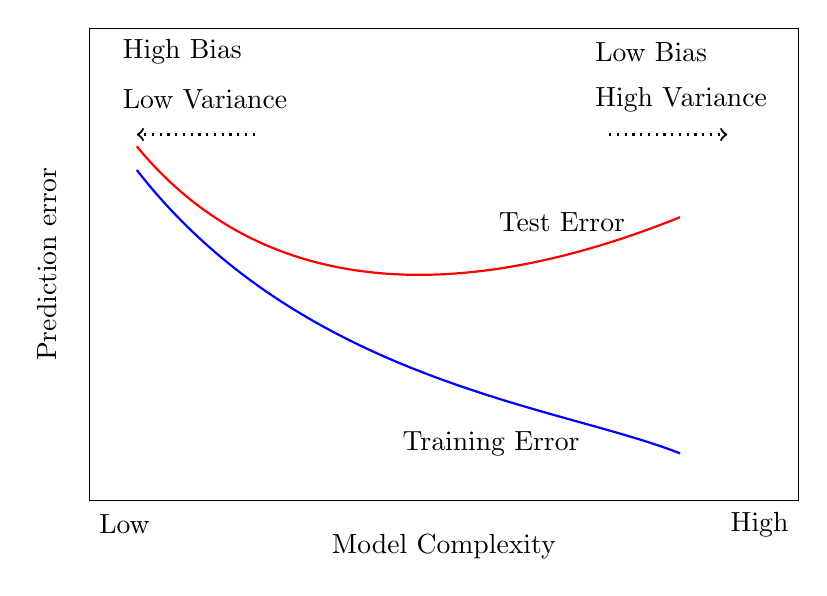
\begin{tikzpicture}[scale=3]
        \draw[] (0,0) rectangle (3,2);
        \draw[red, thick] (0.2,1.5) .. controls (0.9,0.65) and (2,1) .. (2.5,1.2);
        \draw[blue, thick] (0.2,1.4) .. controls (0.9,0.5) and (2,0.4) .. (2.5,0.2);
        \draw[->, dotted, thick] (0.7,1.55)--(0.2,1.55);
        \draw[->, dotted, thick] (2.2,1.55)--(2.7,1.55);
        \node[anchor=south] at (2,1.1) {Test Error};
        \node[anchor=south] at (1.7,0.15) {Training Error};
        \node[anchor=west] at (2.1,1.9) {Low Bias};
        \node[anchor=west] at (2.1,1.7) {High Variance};
        \node[anchor=west] at (0.1,1.9) {High Bias};
        \node[anchor=west] at (0.1,1.7) {Low Variance};
        \node[anchor=west] at (0,-0.1) {Low};
        \node[anchor=east] at (3,-0.1) {High};
        \node[anchor=south, rotate= 90] at (-0.1,1) {Prediction error};
        \node[anchor=north] at (1.5,-0.1) {Model Complexity};
    \end{tikzpicture}
    \fi
    \caption[Model complexity vs prediction error]{Illustration of how an increase in model complexity does not necessarily mean a lower prediction error when tested on new data. Thus, this can also be seen as an illustration of the Bias-Variance trade-off in model selection.}
    \label{fig:model_complexity}
\end{figure}

In search for the optimal model with the right complexity, one can constrain the hypothesis space to some extent.\footnote{The full hypothesis space is the space of all models ${f:\mathbb{R}^M \to \mathbb{R}}$, where $M$ is the number of features in the feature vector} For the sake of example, one could assume a linear relationship between the attributes, i.e., assuming that a target $y$ can be modelled as linear combinations of the features with weights $\bsw$ \eqref{lin_relation} 
\begin{equation}\label{eq:lin_relation}
    f\qty(\xxx,\bsw)  =  \xxx^{\top} \bsw  +w_0 
\end{equation} 

and thereby constrain the hypothesis space to the space of linear models.
In the supervised learning regime illustrated in \figref{supervised_learning}, we try to model inputs $\xxx$ to given outputs $y$, 
\begin{align}\label{eq:supervised_modelling}
    y&=f\qty(\xxx,\bsw) + \varepsilon
\end{align}
Where the modelling function $f\qty(\xxx,\bsw)$ is a function of the fixed feature vector $\xxx$ where the weights of the individual attributes are given as $\bsw$. The $\varepsilon$ parameter represents an unknown error term due to noise. The learning part of these supervised methods is then to optimize the weights based on the data set $\mathcal{D}$ in order to predict new observations accurately. Due to the results of this project being produced by a linear regression model, further elaboration of the linear regression model is considered appropriate.

\subsubsection{The Linear Regression Model}
The linear model assumes the targets $\yyy$ can be modelled as a linear function of the feature vector $\xxx$. Assuming that the data has been standardized (centered), the linear model are given as 
\begin{equation}\label{eq:lin_standard}
    f\qty(\xxx,\bsw) = \xxx^{\top} \bsw
\end{equation}

When trying to fit a proper model according to the machine learning method described in \secref{mlmethod}, one will then attempt to optimize the weights by minimizing a dissimilarity measure. The dissimilarity measure/error function used for the linear regression model is the residual sum of squares\index{Residual Sum of Squares} and the optimization \index{Optimization}problem is given as, 
\begin{equation}
    \bsw^* = \argmin_{\bsw} \curlyb{E\qty(\bsw)} = \argmin_{\bsw} \curlyb{\sum_{i=1}^{N} \qty(\hat{y}_i-\xxx^{\top} \bsw)^2}
\end{equation}
and with analysis, $\bsw^*$ can be found in terms of the data matrix $\XXX$ and the targets $\yyy$ as
\begin{equation}\label{eq:non_penalized_lin_model}
    \bsw^* = \qty( \XXXtilde^{\top} \XXXtilde )^{-1} \XXXtilde^{\top} \yyy
\end{equation}
Derivations of these results can be found in \appref{derivations}. 

\subsection{Penalization of the linear regression model}\label{sec:linmodel}
\index{Ordinary Least Squares}\index{Residual Sum of Squares}\index{Penalization}
As earlier stated, the linear regression model assumes that the targets can be predicted by linear combinations of the attributes of $\xxx$, which takes the form of \eqref{lin_relation}.   
The \emph{Ordinary Least Squares} (OLS) method is a linear regression model utilizing that the optimization of the weights is done using the \emph{residual sum of squares} (RSS) as the error function. The optimal weights $\bsw^*$ is then obtained by minimizing the residual sum of squares with respect to the weight vector\footnote{Again assuming that the data is centered, so that the bias weight $w_0$ can be neglected.}, $\bsw$, \begin{equation}\label{eq:ordinary_least_squares}
    \begin{split}
    \bsw^{*} = \argmin_{\bsw} \left\{\mathrm{RSS}\qty(\bsw) \right\} &= \argmin_{\bsw} \left\{ \sum_{i=1}^{N} \qty(\hat{y}_i - f\qty(\xxx_i))^2 \right\}\\
    &=\argmin_{\bsw} \left\{ \sum_{i=1}^{N} \qty( \hat{y}_i - \xxx^{\top} \bsw)^2 \right\}
    \end{split}
\end{equation}
A nice property of the linear regression is that it can be arbitrarily complex and take non-linear relations into account by introducing feature transformations, described in \secref{dataprep}, i.e., one can account for non-linear relationships by introducing feature transformations such as squaring the initial attributes. These feature transformations can exploit other proportionalities between the feature vectors and targets, but they increase the model complexity \index{Model Complexity} as well, which might result in overfitting the data. Thus, the optimization problem can be restated as finding the perfect balance between bias and variance, as illustrated in \figref{model_complexity}. The \emph{bias-variance trade-off} can be taken into consideration by penalizing the error function. Examples of such penalizations are the Lasso and the Ridge regressions. The benefits of applying coefficient shrinkage like Lasso\index{Lasso} and Ridge \index{Ridge Regression}is not just the consideration of the bias-variance trade-off\index{Bias-Variance Trade-off}, but both regression\index{Regression} types also increase the interpretability of a given model due to the fact that they allow weights for irrelevant attributes to shrink towards zero.

\subsubsection{Least Absolute Shrinkage and Selection Operator (Lasso)}
Like OLS, Lasso optimizes the residual sum of squares with respect to the weights, but adds the constraint that the sum of absolute values of weights should be less or equal to some shrinkage parameter $s$ which has to be chosen appropriately. Thus the formal formulation for the Lasso method is as \eqref{ordinary_least_squares} under the extra constraint that,
\begin{equation}\label{eq:lasso_shrinkage_constraint}
\sum_{j=1}^{M} \left| w_j \right| \leq s
\end{equation}
If the $s$ parameter is less than the full OLS estimate, this penalization will cause the weights of less important attributes to shrink until some truncate at $w_k=0$ is reached in order to fulfill \eqref{lasso_shrinkage_constraint}. This is equivalent to the problem of minimizing: 
\begin{equation}\label{eq:lasso_prob}
    \bsw^{*} = \argmin_{\bsw} \left\{ \sum_{i=1}^{N} \qty(y_i -\bsw^{\top} \xxx_i)^2 + \lambda \sum_{j=1}^{M} \left| w_j \right| \right\}
\end{equation}
where the value of $\lambda$ indicates the amount of shrinkage, i.e., a bigger value of $\lambda$ implies more shrinkage and thus more bias added to the model and vice versa with smaller values of $\lambda$ which means that less bias is introduced.\footnote{$\lambda$ is generally referred to as the regularization strength and usually takes on values in the range of $10^{-5}$ to 1.} Regularization is thus a method of substantially reducing the variance of a model without introducing too much bias if $\lambda$ is chosen wisely. The concepts of regularization arises naturally from probability theory by acknowledging that the prior probability distribution of the weights, $p\qty(\bsw)$ is not supposed to be ignored/assumed uniform in the derivation of the OLS.\footnote{However, proof of this statement will not be included in this project, but can be found in a lot of literature, e.g. \citep{allhailkingMorten}}


\paragraph{The difference between Lasso and Ridge} lies in the \Lnorm{p} used to penalize the residual sum of squares. Whereas Lasso uses the \Lnorm{1}, Ridge regression regularizes using a \Lnorm{2}.\footnote{This results in the solutions to the optimization problem for Lasso being non-linear in $y$ while the solutions to the Ridge optimization problem is linear in $y$} To understand the difference between the two penalization types, the geometry of Lasso and Ridge will be studied briefly using the OLS criterion which is equivalent to the quadratic function,
\begin{align}
    \qty(\bsw - \bsw^0)^{\top} \XXXtilde^{\top} \XXXtilde (\bsw - \bsw^0)+C
\end{align}
where $\bsw^0$ is the full OLS estimate without shrinkage and $C$ is a constant. In \figref{lassovsridge}, the contours of this quadratic function are outlined as well as the constraint regions for the Lasso ($L_1$-norm) and Ridge ($L_2$-norm) respectively. In the two dimensional case of \figref{lassovsridge} it is seen that the contours can hit the tip of the constraint region in the Lasso case. If this happens, one of the two weights will become equal to zero. In the Ridge case, the weights can only become $\approx 0$. This two dimensional example can easily be expanded and hence the Lasso allows for sparse solutions in regards to the number of features. 

The decision about whether to apply a Lasso- or Ridge penalization, as usual, requires the machine learning practitioner to think about the data set in hand. According to the results found by \citep{Tibshirani94regressionshrinkage}, the Ridge penalization is performing better than Lasso when the target values can be predicted by many small effects, whereas Lasso performs best when there is a small to moderate number of features that contribute to predict the targets, as \figref{lassovsridge} suggests as well.

In this project, we would like to create an as low dimensional feature vector as possible, i.e. look for the smallest set of features being able to predict the targets of our model fairly accurately. Hence, the \Lnorm{1} seems like the preferable choice of regularization. However, since we would like to find the smallest possible set of features able to predict our targets, it is worth considering sequential feature selection.\index{Sequential Feature Selection}\index{Forward Selection}

\paragraph{Forward selection} iterates through the features one by one and adds the feature with the lowest test error $E_{\mathrm{test}}$ to the optimal set of features. It then tries to add another feature to the feature vector by searching for candidates that can lower the error compared to the single feature. If multiple features can lower $E_{\mathrm{test}}$, the one that results in the largest decrease in test error will be chosen. The algorithm then continues until the test error cannot be decreased by addition of another feature. According to \citep{Tibshirani94regressionshrinkage}, this method is preferable when there is a small amount of large effects, i.e. a small amount of highly important features.
%%%%%%%%%%%%%%%%%%%%%%%%%%%%%%%%%%%
%   Lasso vs Ridge penalty plot   %
%%%%%%%%%%%%%%%%%%%%%%%%%%%%%%%%%%%

\begin{figure}[t]
    \centering
    %First pictures
   
    \begin{subfigure}[b]{0.45\textwidth}
    \iffigure
        \begin{tikzpicture}
            \begin{axis}[no markers,xlabel=$\hat{w}_1$, 
                ylabel=$\hat{w}_2$,
                ticks=none,
                axis x line=center,
                axis y line=center,
                ymin=-1.1,
                xmin=-1.1,
                xmax=2,
                ymax=3,
                axis equal]
                \addplot+[fill=softblue, color=softblue, opacity=0.5] coordinates
                {(-1,0) (0,1) (1,0) (0,-1)}--cycle;
                \draw[red] (1,2) ellipse [x radius=0.4, y radius=0.2, rotate=45];
                \draw[red] (1,2) ellipse [x radius=0.6, y radius=0.3, rotate=45];
                \draw[red] (1,2) ellipse [x radius=1, y radius=0.5, rotate=45];
                \draw[red] (1,2) ellipse [x radius=1.4, y radius=0.7, rotate=45];
                \node[] at (1,2) {$\hat{w}$};
            \end{axis}
            %
        \end{tikzpicture}
        \fi
    \end{subfigure}
    \quad
    %Second picture
    \begin{subfigure}[b]{0.45\textwidth}
    \iffigure
        \begin{tikzpicture}
            \begin{axis}[no markers,xlabel=$\hat{w}_1$, 
                ylabel=$\hat{w}_2$,
                ticks=none,
                axis x line=center,
                axis y line=center,
                ymin=-1.1,
                xmin=-1.1,
                xmax=2,
                ymax=3,
                axis equal]
                \filldraw[draw=softblue, fill=softblue, opacity=0.5] (0,0) circle (1);
                \draw[red] (1,2) ellipse [x radius=0.4, y radius=0.2, rotate=45];
                \draw[red] (1,2) ellipse [x radius=0.6, y radius=0.3, rotate=45];
                \draw[red] (1,2) ellipse [x radius=1, y radius=0.5, rotate=45];
                \draw[red] (1,2) ellipse [x radius=1.3, y radius=0.65, rotate=45];
                \node[] at (1,2) {$\hat{w}$};
            \end{axis}
        \end{tikzpicture}
        \fi
    \end{subfigure}
    
    \caption[Lasso versus Ridge Shrinkage]{Illustration of how the Least Absolute Shrinkage and Selection Operator (Lasso) is able to set some weights of features to 0 (using the \Lnorm{1}) whereas Ridge regression only allow specific feature weights to be $\approx$ 0 but $\neq$ 0 (using the \Lnorm{2}). The figure on the left shows a \Lnorm{1} and on the right a \Lnorm{2}.}
    \label{fig:lassovsridge}
\end{figure}

%%%%%%%%%%%%%%%%%%%%%%%%%%%%%%%%%%%%

\seclab{Model selection and performance Evaluation}{mspe}\index{Model Selection}\index{Performance Evaluation}
When performing model selection, one should assess the optimal model as the model which generalizes best to unseen data, i.e., to search for the model that will minimize the test error curve in \figref{model_complexity}. But the test error is specific to a given test, hence, to get the true prediction error, one would like to test the model on as much unseen data as possible and ideally, an infinite amount of data. The generalization error, which is an idealized quantity, is introduced as the error the model would have, had it been tested on an infinite amount of test data $\notin$ $\mathcal{D}_{\mathrm{train}}$.

\subsection{Cross-validation}\label{sec:crossvalidation}\index{Cross-Validation}

\begin{figure}[ht]
    \centering
    \iffigure
    \begin{tikzpicture}
    
        %First line
        \filldraw[draw=softblue, fill=softblue] (0,3.5) rectangle (12,4.5);
        % third line
        \filldraw[draw=softblue, fill=softblue] (0,2) rectangle (12,3);
        \filldraw[draw=softgrey, fill=softgrey] (0,2) rectangle (4,3);
        %fourth line
        \filldraw[draw=softblue, fill=softblue] (0,0.5) rectangle (12,1.5);
        \filldraw[draw=softgrey, fill=softgrey] (4,0.5) rectangle (8,1.5);
        %fith line
        \filldraw[draw=softblue, fill=softblue] (0,-1) rectangle (12,0);
        \filldraw[draw=softgrey, fill=softgrey] (8,-1) rectangle (12,0);
        %Legend
        \node[] at (6,4) {$N$};
        
        \node[] at (2,2.5) {$\dfrac{1}{3}N$ };
        \node[] at (8,2.5) {$\dfrac{2}{3}N$ };
        
        \filldraw[draw=softblue, fill=softblue] (0,5) rectangle (0.5,5.5);
        \node[anchor=west] at (0.5,5.25) {Training data};
        
        \filldraw[draw=softgrey, fill=softgrey] (9.5,5) rectangle (10,5.5);
        \node[anchor=west] at (10,5.25) {Test data};
        
        
    \end{tikzpicture}
    \fi
    \caption[Cross-validation illustration]{Visual example of $K$-fold CV; Here seen a 3-fold validation where the data set is split into subsets, $\mathcal{D} = \mathcal{D}_1 \cup \mathcal{D}_2 \cup \mathcal{D}_3 $. For each subset, the model is trained on 2/3 and tested on 1/3 of the total $N$ observations.}
    \label{fig:kfold}
\end{figure}


\emph{Cross-validation} (CV) is a technique which beautifully takes into account, that when finding the optimal model for a problem, one must not test the model on the data used for training. The idea behind CV, is to create as much test and training data using only the data set itself. There are three major types of cross-validation, \emph{Hold-Out} CV, \emph{K}-fold CV and \emph{Leave-one-out} Cross-validation\citep{allhailkingMorten}. In this project, \emph{K}-fold has been used exclusively. Both for model selection and estimating the generalization error of the optimal model. When performing $K$-fold CV, the data set is split into $K$ subsets, $\mathcal{D} = \mathcal{D}_1 \cup  ... \cup \mathcal{D}_k \cup ... \cup \mathcal{D}_K$. Hence, $K$-fold CV allows one to test the models on the entire data set.

In $K$-fold CV, the idealized generalization error \index{Generalization Error} is approximated as:
\begin{equation}\label{eq:gen_error}
    \EM{gen} \approx \sum_{k=1}^K \dfrac{N_{k}^{\mathrm{test}}}{N}   E_{\mathcal{M},k}^{\mathrm{test}}
\end{equation}
where $N_k^{\mathrm{test}}$ is the number of observations for testing in fold number $k$, and $\EMss{,k}{test}$ is given as
\begin{equation}
    \EMss{,k}{test} = \dfrac{1}{N_{k}^{\mathrm{test}}} \sum_{i \in \Dtest} d\qty(y_i,\FM{\xxx_i,\bsw})
\end{equation}
The appropriate dissimilarity measure varies from task to task, but recall that in the case of regression, one uses the RSS. An illustrative example of how the data is split for a $3$-fold CV is seen in \figref{kfold}.

CV can be used for both model selection and estimation of the generalization error. Two-layer CV is a way of doing both and thus getting an unbiased estimate of the generalization error. This is done for every model created in the code phase of this project. Therefore the procedure is outlined in pseudo-code in Algorithm \ref{algo:tlcv}\footnote{The idea of outlining the Algorithm in pseudo-code is due to \citep{allhailkingMorten}}.
\begin{algorithm}
\caption{$K$-Fold Cross-Validation for Model selection and $\EM{gen}$ estimation}

\begin{algorithmic}[0]

\Require{$K_1$ folds in outer loop for estimation of the generalization error}
\Require{$K_2$ folds in inner loop for model selection}
\Require{$S$ models to cross-validate: $\mathcal{M}_1 , ... , \mathcal{M}_S$}
\Ensure{$\hat{E}_{\mathcal{M}*}^{\mathrm{gen}}$}

\For{$i =1,...,K_1$}
    \State{\emph{Outer CV loop. The data set, $\calD$ is split into $K_1$ folds} }
    \State{The $i$'th split of $\calD$ is $\calD_{i}^{\mathrm{par}},\calD_{i}^{\mathrm{test}}$}
    \For{$j=1,...,K_2$}
        \State{\emph{Inner CV loop doing $K_2$ splits for model selection testing $S$ models}}
        \State{The $j$'th split of $\calD_i^{\mathrm{par}}$ is $\calDss{j}{train},\calDss{j}{val}$} 
        \For{$s=1,...,S$}
            \State{Train $\mathcal{M}_s$ on $\calDss{j}{train}$ }
            \State{Let $\EMss{_{s,j}}{val}$ be the \emph{validation error} of the model $\mathcal{M}_s$ when it is \emph{tested} on $\calDss{j}{val}$}
        \EndFor
    \EndFor    
    \State{For each $s$ compute $\hat{E}_s^{\mathrm{gen}}= \sum_{j=1}^{K_2} \frac{\abs{\calDss{j}{val}}}{\calDss{i}{par}} \EMss{_s,j}{val}$ }
    \State{Select the optimal model $\mathcal{M}^*$ = $\mathcal{M}_{s^*}$ where $s^* = \argmin_s \hat{E}_s^{\mathrm{gen}}$}
    \State{Train $\mathcal{M}^*$ on $\calDss{i}{par}$}
    \State{Let $E_i^{\mathrm{test}}$ be the \emph{test error} of the model $\mathcal{M}^*$ when it is tested on $\calDss{i}{test}$}
\EndFor
\State{Compute the estimate of the generalization error: $\hat{E}^{\mathrm{gen}} = \sum_{i}^{K_1} \frac{\abs{\calDss{i}{test}}}{N} E_i^{\mathrm{test}}$}
\end{algorithmic}
\label{algo:tlcv}
\end{algorithm}








\chapter{Machine learning in physics}\label{chap:ml_in_physics}
\thispagestyle{empty}
%%%%%%%%%%%%%%%%%%%%%%%%%%%%%%%%%%%%%%%%%%%%%%%%%%%%%
%   Chapter 2: OUTLINE                              %
%%%%%%%%%%%%%%%%%%%%%%%%%%%%%%%%%%%%%%%%%%%%%%%%%%%%%
Quantum simulation methods like density functional theory and quantum Monte Carlo simulations have facilitated accurate calculations of quantum systems. The amount of quantum simulations performed on a daily basis is immense, but these methods have their restrictions. The time consumption of a DFT simulation increases significantly with the amount of atoms, i.e. $T\sim N^{\alpha}$ with $\alpha \approx 2-3$ and $N$ the number of atoms \citep{KohnNobelLecture}. Thus, if one could predict different material properties more efficiently it would be beneficial to the field of material sciences. The tools of machine learning bring possibilities of doing just that. For example, the situation where a group has done extensive research with quantum simulations on a system of interest. The data achieved by performing these computationally costly simulations can with proper ML methods promote knowledge about the systems of interest as illustrated in \figref{mlandquant}. The figure illustrates how ML can contribute to material sciences by learning from quantum simulated data and additional knowledge about the systems. 
\begin{figure}[ht]
    \centering
    %\iffigure
        \begin{tikzpicture}

        \filldraw[fill=softblue, draw=softblue,ultra thick, rounded corners=15pt, opacity=0.5 ] (-3.5,0.5) rectangle (3.5,2);
        \filldraw[fill=softblue, draw=softblue,ultra thick, rounded corners=15pt, opacity=0.5] (-3.5,-2) rectangle (3.5,-0.5);
        \filldraw[fill=softblue, draw=softblue,ultra thick, rounded corners=15pt, opacity=0.5] (-3.5,-4.5) rectangle (3.5,-3);
        \draw[ultra thick,->, rounded corners=15pt] (3.5,-3.75)--(4.5,-3.75)--(4.5,1.25)--(3.5,1.25);
        \draw[->, ultra thick] (0,0.5)--(0,-0.5);
        \draw[->, ultra thick] (0,-2)--(0,-3);
        
        \node[] at (0,1.25) {Systems of interest (SOI)};
        
        \node[] at (0, -1.25) {Data to be used for ML};
        \node[] at (0,-3.75) {ML model for predictions, $\hat{y}$};
        \node[anchor=south east] at (0,-0.5) {QM computation};
        \node[anchor=south east] at (0,-3) {ML algorithm};
        \node[anchor=west] at (4.5,-1.25) {\rotatebox[origin=c]{270}{Supplementary understanding of SOI}};
    \end{tikzpicture}
    %\fi
    \caption[Machine learning and Quantum Computations]{Illustration of how quantum theory and machine learning can help each other in predicting properties of materials. Machine learning can help speed up the computations by predicting and validating the best candidates as the computation provides raw data for the machine learning model to train on. }
    \label{fig:mlandquant}
\end{figure}
The thoughts about ML and material sciences has consequently brought a lot of attention to the subject and therefore a quick review of the already implemented methods is considered convenient.

\seclab{Implemented ML methods in materials science}{donesofar}

 Several approaches to utilize machine learning algorithms in material science and physics have been made in recent times \citep{mueller_kussesne,criticalrole_descriptor,frameworkforML}. The approaches include predictions of phase diagrams \citep{phasediagram,phase2diagrams}, predictions of various material properties based on data from quantum mechanical computations \citep{rupp,Pilania2013}, interatomic potentials development \citep{hansen2015a,huan2015a, bartok2010a, behler2011a, behler2007a}, predictions of crystal structures  \citep{woodley2008a,madoxx1988,fischer2006a}, discovering and developing density functionals \citep{behler2011ANN}, modelling of crystal lattices \citep{mueller2009a, mueller2012a, seko2009a} along with behavior and processing of complex materials \citep{metzbower2001a, bucholz2012a}.
While some of these are somewhat out of the scope of this project they resemble what can be achieved using machine learning as an asset to established methods in materials science and engineering. An approach related to the procedure of this project was performed by \emph{Rupp et al.} \citep{rupp} who used a ridge regression with a Gaussian Kernel to predict accurate molecular atomization energies. Their data set, which was calculated with\index{Density Functional Theory} (DFT), contained more than 7000 organic molecules, each consisting of up to 7 atoms and they achieved a \emph{Root Mean Squared Error} (RMSE) of $\approx$ 1.3 eV per molecule and a \emph{Mean Absolute Arror} of $\approx$ 0.65 eV per molecule for the machine learning method. 
Another study closely related to this project \citep{criticalrole_descriptor} investigates how to use the Lasso \index{Lasso} method for feature selection in order to predict the difference in energies for two different structures of binary compounds. The purpose of their studies was to outline the critical role of using a suitable feature vector and investigates if a low-dimensional representation of the feature vector would be able to predict the target values. The data set used by \emph{Ghiringhelli} and \emph{Scheffler} consists of 82 binary octet materials, $N=82$, with the target values $\yyy$ = \emph{"The energy differences between the rock salt crystal structure and the zinc blende or wurtzite structures"}. We will strive to do something similar in this project, however, being able to find as low-dimensional feature vectors is unlikely, due our model being more complex as non-octet sets are considered. 
Among all the different ways to implement machine learning in materials science, using the Lasso can serve as a suitable method, since one can create arbitrarily complex feature transformations in accordance to \secref{dataprep} and then penalize the model to reduce complexity to the right amount by using CV for model selection. By doing so, one can introduce the right amount of bias and variance to create a well-generalizing model which keeps its interpretability intact.

\seclab{Predicting the difference in heat of formation between four crystal structures}{main_model}\index{Heat of Formation}\index{Crystal Structures}
%We are living in a time where a lot of research in materials sciences focus on exploration of materials with specific properties for specific purposes. For example, the search for possible materials to be utilized in photovoltaic solar cells. In such a search, it is common to start with a screening phase where a lot of potential candidates are discarded. Even though computer science has evolved a lot in recent years and we can run computationally expensive molecular simulations, methods like DFT and Quantum Clustering can be considered inefficient in such screening processes as they are computationally too costly for the purpose.
The hope of this project is to create a machine learning model able to contribute to the current goals of materials science. Ideally, through the modelling of this project, we can create a universal set of features being able to accurately predict which of the considered crystal structures is the most stable. By doing so, one could reduce the amount of more advanced quantum simulations significantly. 
\subsection{The crystal structures used in the project}
\begin{table}[ht]
    \centering
    \begin{tabular}{cccccc}
    \toprule
    Kind of atom  & \multicolumn{4}{c}{Atom} \\\midrule
    \multirow{11}{*}{\textbf{A}} 
        & Li & Be & B & Na  \\
        & Mg & Al & Si & K  \\
        & Ca & Sc & Ti & Zn \\
        & Ga & Ge & As & Rb  \\ 
        & Sr & Y & Zr & Nb  \\
        & Mo & Ru & Rh & Pd  \\
        & Ag & Cd & In & Sn  \\
        & Sb & Te & Cs & Ba  \\
        & La & Hf & Ta & Re  \\
        & Os & Ir & Pt & Au  \\\midrule
    \multirow{4}{*}{\textbf{B}}    
        & B & C & N & O   \\
        & F & Si & P & S   \\
        & Cl & Ge & As & Se   \\
        & Br & Sb & Te & I   \\\bottomrule
    \end{tabular}
    \caption[The different A and B atoms used]{Identification of the different A and B atoms used to construct the dimers. As seen, there are $44 \times 16 = 704$ different combinations, given us 704 rows of data to be used for machine learning.}
    \label{tab:ABcompounds}
\end{table}

This project has examined four different data sets. Each data set containing the heat of formation, $\Delta H$ of AB compounds calculated with DFT for different crystal structures. The four different structures examined are \emph{Rock Salt} (Rs), \emph{Nickel Arsenide} (NiAs), \emph{Zinc Blende} (Zb) and \emph{Wurtzite} (Wz) and unit cells for each can be seen on \figsref{rs}{nias}{zb}{wz}. In each of the four data sets, there are 44 different A atoms and 16 different B atoms and the data sets contain every combination of A and B. This gives a total of $N = 44 \times 16 = 704$ observations; the different A and B atoms are outlined in \tabref{ABcompounds}.

To get the most data out the model, a machine, that via. a reference structure is able to predict the energy differences between all of the four crystal structures using a multi-target regression, is to prefer. If such a model can be constructed, one would be able get a lot of information out of a a single feature vector $\xxx_i$. 

The target values for the different models that will be constructed is thus, 
\begin{align}
  \hat{y} = \Delta H_{cs \neq r} - \Delta H_{r}  
\end{align}
i.e., if the reference structure as an example is Rock Salt, then $\Delta H_{r} = \Delta H_{\mathrm{Rs}}$ and $\Delta H_{cs \neq r} = \curlyb{\Delta H_{\mathrm{NiAs}},\Delta H_{\mathrm{Zb}},\Delta H_{\mathrm{Wz}}}$
\begin{figure}
    \begin{subfigure}[b]{0.45\textwidth}
    \centering
    \iffigure
    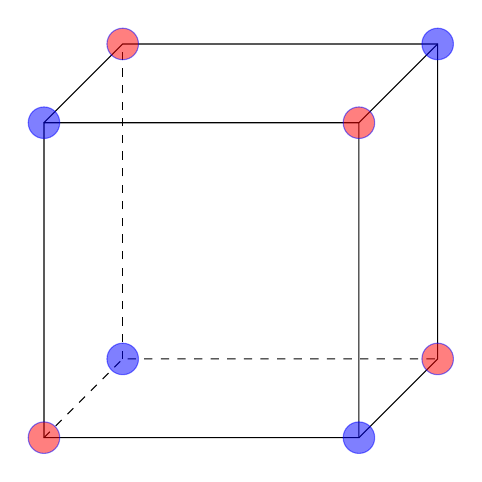
\begin{tikzpicture}
    %Firkant
        \draw[] (0,0) rectangle (4,4)--(5,5);
        \draw[] (0,4)--(1,5)--(5,5)--(5,1)--(4,0);
        \draw[dashed] (0,0)--(1,1)--(5,1) ;
        \draw[dashed] (1,1)--(1,5);

    %Atomer    
        \filldraw[fill=red, draw=blue,opacity=0.5] (0,0) circle (0.2);
        \filldraw[fill=blue, draw=blue,opacity=0.5] (4,0) circle (0.2);
        \filldraw[fill=blue, draw=blue,opacity=0.5] (0,4) circle (0.2);
        \filldraw[fill=red, draw=blue,opacity=0.5] (4,4) circle (0.2);
        \filldraw[fill=blue, draw=blue,opacity=0.5] (1,1) circle (0.2);
        \filldraw[fill=red, draw=blue,opacity=0.5] (5,1) circle (0.2);
        \filldraw[fill=red, draw=blue,opacity=0.5] (1,5) circle (0.2);
        \filldraw[fill=blue, draw=blue,opacity=0.5] (5,5) circle (0.2);
        
        %
    \end{tikzpicture}
    \fi
    \caption{Crystal Structure of Rock Salt (RS). }
    \label{fig:rs}
    \end{subfigure}
    %
    \quad
    %
    \begin{subfigure}[b]{0.45\textwidth}
    \centering
    \iffigure
    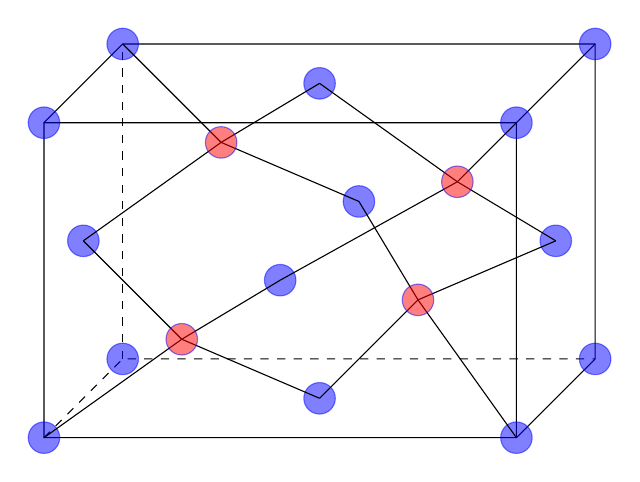
\begin{tikzpicture}
    %Firkant
        \draw[] (0,0) rectangle (6,4)--(7,5);
        \draw[] (0,4)--(1,5)--(7,5)--(7,1)--(6,0);
        \draw[dashed] (0,0)--(1,1)--(7,1) ;
        \draw[dashed] (1,1)--(1,5);

    %Atomer    
        \filldraw[fill=blue, draw=blue,opacity=0.5] (0,0) circle (0.2);
        \filldraw[fill=blue, draw=blue,opacity=0.5] (6,0) circle (0.2);
        \filldraw[fill=blue, draw=blue,opacity=0.5] (0,4) circle (0.2);
        \filldraw[fill=blue, draw=blue,opacity=0.5] (6,4) circle (0.2);
        \filldraw[fill=blue, draw=blue,opacity=0.5] (1,1) circle (0.2);
        \filldraw[fill=blue, draw=blue,opacity=0.5] (7,1) circle (0.2);
        \filldraw[fill=blue, draw=blue,opacity=0.5] (1,5) circle (0.2);
        \filldraw[fill=blue, draw=blue,opacity=0.5] (7,5) circle (0.2);
        %
        \filldraw[fill=blue, draw=blue,opacity=0.5] (0.5,2.5) circle (0.2);
        \filldraw[fill=blue, draw=blue,opacity=0.5] (6.5,2.5) circle (0.2);
        \filldraw[fill=blue, draw=blue,opacity=0.5] (3,2) circle (0.2);
        \filldraw[fill=blue, draw=blue,opacity=0.5] (4,3) circle (0.2);
        \filldraw[fill=blue, draw=blue,opacity=0.5] (3.5,0.5) circle (0.2);
        \filldraw[fill=blue, draw=blue,opacity=0.5] (3.5,4.5) circle (0.2);
        %
        \draw[thin] (0,0)--(1.75,1.25);
        \draw[thin] (0.5,2.5)--(1.75,1.25);
        \draw[thin] (3,2)--(1.75,1.25);
        \draw[thin] (3.5,0.5)--(1.75,1.25);
        
        \draw[thin] (3.5,0.5)--(4.75,1.75);
        \draw[thin] (4,3)--(4.75,1.75);
        \draw[thin] (6,0)--(4.75,1.75);
        \draw[thin] (6.5,2.5)--(4.75,1.75);
        
        \draw[thin] (1,5)--(2.25,3.75);
        \draw[thin] (0.5,2.5)--(2.25,3.75);
        \draw[thin] (3.5,4.5)--(2.25,3.75);
        \draw[thin] (4,3)--(2.25,3.75);
        
        \draw[thin] (3,2)--(5.25,3.25);
        \draw[thin] (3.5,4.5)--(5.25,3.25);
        \draw[thin] (6,4)--(5.25,3.25);
        \draw[thin] (6.5,2.5)--(5.25,3.25);
        %
        \filldraw[fill=red, draw=blue,opacity=0.5] (2.25,3.75) circle (0.2);
        \filldraw[fill=red, draw=blue,opacity=0.5] (1.75,1.25) circle (0.2);
        \filldraw[fill=red, draw=blue,opacity=0.5] (5.25,3.25) circle (0.2);
        \filldraw[fill=red, draw=blue,opacity=0.5] (4.75,1.75) circle (0.2);
    \end{tikzpicture}
    \fi
    \caption{Crystal structure of Zinc blende (ZB).}
    \label{fig:zb}
    \end{subfigure}
    \\
    \begin{subfigure}[b]{0.45\textwidth}
    \centering
    \iffigure
    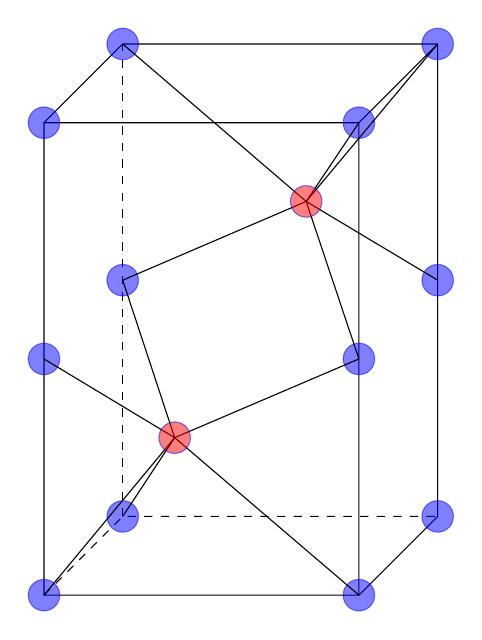
\begin{tikzpicture}
    %Firkant
        \draw[] (0,0) rectangle (4,6)--(5,7);
        \draw[] (0,6)--(1,7)--(5,7)--(5,1)--(4,0);
        \draw[dashed] (0,0)--(1,1)--(5,1) ;
        \draw[dashed] (1,1)--(1,7);
   \iffalse
    %Koordinatsystem
        \draw[thick,->] (-3,0)--(-1,0);
        \draw[thick,->] (-3,0)--(-2.5,0.5);
        \draw[thick,->] (-3,0)--(-3,2);
        \node[anchor=west] at (-1,0) {$x$};
        \node[anchor=west] at (-2.5,0.5) {$y$};
        \node[anchor=west] at (-3,2) {$z$};
    \fi
    %Atomer    
        \filldraw[fill=blue, draw=blue,opacity=0.5] (0,0) circle (0.2);
        \filldraw[fill=blue, draw=blue,opacity=0.5] (4,0) circle (0.2);
        \filldraw[fill=blue, draw=blue,opacity=0.5] (0,3) circle (0.2);
        \filldraw[fill=blue, draw=blue,opacity=0.5] (4,3) circle (0.2);
        \filldraw[fill=blue, draw=blue,opacity=0.5] (1,1) circle (0.2);
        \filldraw[fill=blue, draw=blue,opacity=0.5] (5,1) circle (0.2);
        \filldraw[fill=blue, draw=blue,opacity=0.5] (1,4) circle (0.2);
        \filldraw[fill=blue, draw=blue,opacity=0.5] (5,4) circle (0.2);
        \filldraw[fill=blue, draw=blue,opacity=0.5] (1,7) circle (0.2);
        \filldraw[fill=blue, draw=blue,opacity=0.5] (4,6) circle (0.2);
        \filldraw[fill=blue, draw=blue,opacity=0.5] (5,7) circle (0.2);
        \filldraw[fill=blue, draw=blue,opacity=0.5] (0,6) circle (0.2);
        %
        \draw[thin] (0,0)--(1.66,2);
        \draw[thin] (1,1)--(1.66,2);
        \draw[thin] (0,3)--(1.66,2);
        \draw[thin] (1,4)--(1.66,2);
        \draw[thin] (4,0)--(1.66,2);
        \draw[thin] (4,3)--(1.66,2);
        
        \draw[thin] (4,3)--(3.33,5);
        \draw[thin] (5,4)--(3.33,5);
        \draw[thin] (4,6)--(3.33,5);
        \draw[thin] (5,7)--(3.33,5);
        \draw[thin] (1,7)--(3.33,5);
        \draw[thin] (1,4)--(3.33,5);
        %
        \filldraw[fill=red, draw=blue,opacity=0.5] (3.33,5) circle (0.2);
        \filldraw[fill=red, draw=blue,opacity=0.5] (1.66,2) circle (0.2);
        % 
    \end{tikzpicture}
    \fi
    \caption{Crystal structure of Nickel Arsenide (NiAs)}
    \label{fig:nias}
    \end{subfigure}
    %
    \quad
    %
    \begin{subfigure}[b]{0.45\textwidth}
    \centering
    \iffigure
    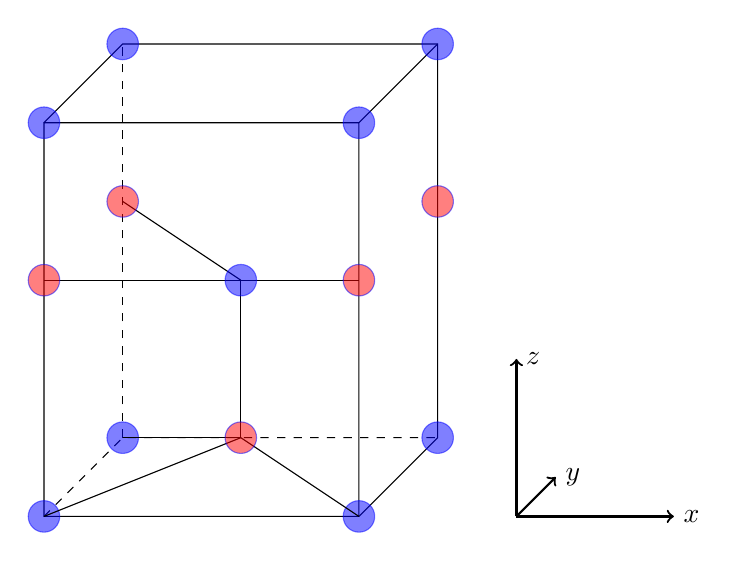
\begin{tikzpicture}
    %Firkant
        \draw[] (0,0) rectangle (4,5)--(5,6);
        \draw[] (0,5)--(1,6)--(5,6)--(5,1)--(4,0);
        \draw[dashed] (0,0)--(1,1)--(5,1) ;
        \draw[dashed] (1,1)--(1,6);

    %Atomer    
        \filldraw[fill=blue, draw=blue,opacity=0.5] (0,0) circle (0.2);
        \filldraw[fill=blue, draw=blue,opacity=0.5] (4,0) circle (0.2);
        \filldraw[fill=blue, draw=blue,opacity=0.5] (0,5) circle (0.2);
        \filldraw[fill=blue, draw=blue,opacity=0.5] (4,5) circle (0.2);
        \filldraw[fill=blue, draw=blue,opacity=0.5] (1,1) circle (0.2);
        \filldraw[fill=blue, draw=blue,opacity=0.5] (5,1) circle (0.2);
        \filldraw[fill=blue, draw=blue,opacity=0.5] (1,6) circle (0.2);
        \filldraw[fill=blue, draw=blue,opacity=0.5] (5,6) circle (0.2);
        %
        \draw[thin] (0,3)--(2.5,3);
        \draw[thin] (1,4)--(2.5,3);
        \draw[thin] (4,3)--(2.5,3);
        
        \draw[thin] (0,0)--(2.5,1);
        \draw[thin] (1,1)--(2.5,1);
        \draw[thin] (4,0)--(2.5,1);
        
        \draw[thin] (2.5,3)--(2.5,1);
        %
        \filldraw[fill=red, draw=blue,opacity=0.5] (0,3) circle (0.2);
        \filldraw[fill=red, draw=blue,opacity=0.5] (1,4) circle (0.2);
        \filldraw[fill=red, draw=blue,opacity=0.5] (4,3) circle (0.2);
        \filldraw[fill=red, draw=blue,opacity=0.5] (5,4) circle (0.2);
        %
        \filldraw[fill=blue, draw=blue,opacity=0.5] (2.5,3) circle (0.2);
        \filldraw[fill=red, draw=blue,opacity=0.5] (2.5,1) circle (0.2);
        
        
      
    %Koordinatsystem
        \draw[thick,->] (6,0)--(8,0);
        \draw[thick,->] (6,0)--(6.5,0.5);
        \draw[thick,->] (6,0)--(6,2);
        \node[anchor=west] at (8,0) {$x$};
        \node[anchor=west] at (6.5,0.5) {$y$};
        \node[anchor=west] at (6,2) {$z$};
    
    \end{tikzpicture}
    \fi
    \caption{Crystal structure of Wurtzite (WZ).}
    \label{fig:wz}
\end{subfigure}

\caption{Unitcells for the four different structures.}
\label{fig:csstruct}
\end{figure}

How the feature vector $\xxx$ for this task has been created, is described in \secref{physicsfeaturevector}.


\subsection{Creating an appropriate feature vector}\label{sec:physicsfeaturevector}
As the desirable feature vector is relatively low-dimensional and our data set containing non-octet compounds is relatively complex, it is very probable that our feature vector should include highly relevant complex attributes. Expert knowledge might come in handy and thus our strategy for creating a suitable feature vector is based on considerations from other people's work, mostly \citep{frameworkforML} and \citep{criticalrole_descriptor}. Initially, a 34-dimensional feature vector is constructed, consisting exclusively of atomic properties of the A- and B atoms and then plenty features will be constructed by feature transformations.

\subsubsection{Atomic attributes}\label{sec:atomic_att}

\pgfplotstableread[col sep=comma] {csv/basic.csv}\basic
\begin{figure}[ht]
    \centering
    \iffigure
    \begin{tikzpicture}
        \begin{axis}[boxplot/draw direction=y,
        xlabel={Attribute}, 
        ylabel={Spread},
        %xtick=data,
        xtick={1,...,17},
        xticklabels={Atom number, Group, Period, Electron negativity, Covalent radius, Atomic radius, Van der Wahls radius, Electron affinity, Ionisation energy, Average oxidation number, Difference in oxidation number, Noble gas, Number of s electrons, Number of p electrons, Number of d electrons, Pettifor radius, Atomization energy pr atom},
        x tick label style={rotate=90,anchor=east},
        enlarge x limits=-1,
        width=1\textwidth,
        height=0.5\textwidth,
        ]
        \foreach \i in {1,...,17} 
            \addplot+[boxplot]
            table[col sep=comma,y index=\i] \basic;
        \end{axis}
    \end{tikzpicture}
    \fi
    \caption[Box-plots for the initial 17 attributes of the A atom]{Boxplot of attributes for the A atom. The data is standardized as described in \secref{statmat}}
    \label{fig:boxplotA}
\end{figure}

\begin{figure}[ht]
    \centering
    \iffigure
    \begin{tikzpicture}
        \begin{axis}[boxplot/draw direction=y,
        xlabel={Attribute}, 
        ylabel={Spread},
        %xtick=data,
        xtick={1,...,17},
        xticklabels={Atom number, Group, Period, Electron negativity, Covalent radius, Atomic radius, Van der Wahls radius, Electron affinity, Ionisation energy, Average oxidation number, Difference in oxidation number, Noble gas, Number of s electrons, Number of p electrons, Number of d electrons, Pettifor radius, Atomization energy pr atom},
        x tick label style={rotate=90,anchor=east},
        enlarge x limits=-1,
        width=1\textwidth,
        height=0.5\textwidth,
        ]
        \foreach \i in {18,...,34} 
            \addplot+[boxplot]
            table[col sep=comma,y index=\i] \basic;
        \end{axis}
    \end{tikzpicture}
    \fi
    \caption[Box-plots for the initial 17 attributes of the B atom]{Boxplot of attributes for the B atom. The data is standardized as described in \secref{statmat}}
    \label{fig:boxplotB}
\end{figure}


\begin{table}[ht]
    \centering
    \begin{tabular}{|p{5cm}|c|l|}\hline
        \textbf{Attribute}                 & \textbf{Unit}  &\textbf{Type}  \\ \hline
        Atom number                 & []    &  Discrete ratio \\ \hline
        Atom group                  & []    &  Discrete ratio \\ \hline
        Atom period                 & []    &  Discrete ratio \\ \hline
        Electron negativity         & [eV]  &  Continuous ratio\\ \hline   
        Covalent radius             & [Å]   &  Continuous ratio \\ \hline
        Atom Radius                 & [Å]   &  Continuous ratio \\ \hline
        Van der Wahls radius        & [Å]   &  Continuous ratio \\ \hline
        Electron affinity           & [eV]  &  Continuous ratio \\ \hline
        Ionisation energy           & [eV]  &  Continuous ratio\\ \hline
        Average oxidation number    & []    &  Continuous ratio\\ \hline 
        Difference between largest and smallest oxidation number & [] & Continuous ratio \\ \hline
        Noble gas number      & []  & Discrete ratio  \\ \hline
        Number of s electrons & []  & Discrete ratio \\ \hline
        Number of p electrons & []  & Discrete ratio \\ \hline
        Number of d electrons & []  & Discrete ratio \\ \hline
        Pettifor radius      & [Å] & Continuous ratio \\ \hline
        Atomization energy per atom  & [eV] & Continuous ratio\\ \hline
    \end{tabular}
    \caption[Overview of the attributes used to describe an atom.]{The 17 attributes loaded from the periodic system used to generate features. The table shows units and attribute types as described in \appref{attribute_types}}
    \label{tab:att}
\end{table}

The atomic attributes in the initial feature vector are outlined in \tabref{att}, but as mentioned in \secref{dataprep}, understanding the data set is crucial. Hence, the following will elaborate on some of the initial attributes. Electron negativity describes the atoms ability to attract another electron, i.e. larger electron negativity means larger attraction. The covalent radius describes the distance an atom would have to another when forming a covalent bond. The atomic radius reflects the ionic radius, which describes the distance to the nearest atom when forming an ionic bond. Another radius to be considered is the Van der Wahls radius. The Van der Wahls radius describes the closest distance one atom can approach another in a hard sphere approximation. Electron affinity describes the cost in energy for adding another electron to the atom in its natural state. The ionization energy is the amount of energy spend to remove the most loosely bounded valence electron. As each atom can have different oxidation numbers the simplest way to describe the amount and size is the average and difference between the largest and smallest. Information about the inner shells of electrons can be found by knowing the noble gasses their atom numbers are listed as an attribute. The outer shells are then described by the number of $s$, $p$ and $d$-electrons in the outer most shell of electrons and the atomization energy is the amount of energy needed to form a mono-atomic gas. Lastly the Pettifor radius is included as an attribute in our feature vector. However, the authors have not been able to find a valid source describing this property. \\

In order to examine the values of the attributes in $\XXXtilde$, two box-plots can be seen in \figtworef{boxplotA}{boxplotB}. In the first figure, \figref{boxplotA}, is shown how the different 17 atomic properties of the A atoms are distributed. Likewise  \figref{boxplotB} has the same visualization purpose for the B atoms. As there are almost three times as many A atoms than B atoms one would expect more variance for the attributes of the A atom, which is the case by comparison of the two figures.\footnote{The observations outside the whiskers occur if they deviate by more than 1.5 $\times$ the interquartile range, measuring from the closest quartile.} It seems like the covalent radius and atomic (or ionic radius) has several observations outside the whiskers for the A atom, while difference in oxidation numbers and number of $p$-electrons each have two. For the B atom the situation is quite different, as there is a single observation outside the whiskers for the Van der Wahls radius, ionisation energy and atomization energy while average oxidation and Pettifor radius each contain two. Overall, the box-plots are in correspondence with what one could expect looking at the list of A and B atoms.


\subsubsection{Feature transformations}\label{sec:featuretrans}\index{Feature Transformations}

As we are ideally trying to predict the difference in heat of formation for the four crystal structures at once, which turns out to be a rather complex task, the initial $M=34$ features might not fit the bill and thus a large number of features are generated from the initial feature vector. As all of the attributes are ratio, the feature transformations can be made arbitrarily complex. 

Most of the initial attributes were loaded with the \texttt{Python}-module \texttt{ELEMENTS} and a few were added from acknowledged databases. The 17 attributes per atom can be seen in \tabref{att} and box-plots for the standardized values\footnote{With respect to the mean and standard deviation of each attribute.} can be found in \figref{boxplotA} and \figref{boxplotB}. The feature vector was then extended by 68 attributes by taking both the natural logarithm and the exponential of each initial attribute, which updated $M=102$ attributes. \\
The idea is to make pairwise linear combinations of different attributes with the same units.\footnote{Energy (eV), Length (Å) and features with no units}
The linear combinations created were:
\begin{itemize}
        \item Sum of pairwise attributes
        \item Absolute value of the difference
        \item The squared sum between 
        \item The difference squared
        \item The exponential values to all of the above.
\end{itemize}
By doing so, we added 288 new features by taking pairwise linear combinations between the \emph{energy} attributes, 168 from the \emph{length} attributes and 1368 from the \emph{no unit} attributes. Therefore, the dimensionality of the feature vector increased to a total of $M=102+288+168+1386=1944$.

The first 102 attributes, i.e. the initial 34 plus the $\log()$ and $\exp()$ to these, were lastly multiplied in every pairwise combination adding $102^2=10404$ features to the 1944 features leaving a $M=12330$ dimensional feature vector ready for modelling.
Hence, since we have $N=704$ AB dimers, the input matrix $\XXX$ contains 704 rows and 12330 columns. \\ In advance of the modelling phase, the data for 32 randomly chosen observations for each crystal structure were put into a secret box with the purpose of final model assessment. We denote this data set, $\mathcal{D}_{\mathrm{test_{box}}}$. The final estimate of relevant erro
 measures is calculated from predictions made on this data set. This leaves us with $N=704-32=672$ observations for training. 

\seclab{The Modelling Phase}{modellingphase}
After creating $\XXX$, one can begin the predictive modelling. As mentioned in \secref{datamodelling}, Lasso will be used exclusively as our modelling method. \\ 
Thus the data matrix $\XXX$, is standardized with respect to the mean and standard deviation of each attribute to construct $\XXXtilde$. If the standard deviation of an attribute is 0, division by the standard deviation of the respective attributes is neglected.

In this section, three different approaches will be examined. In all of these approaches, the heat of formation for the \emph{rock salt} crystal structure was used as reference structure, $\Delta H_{r} = \Delta H_{\mathrm{Rs}}$. Other than having the same reference structure, the different approaches are similar in numerous ways. First and foremost, the models work in an iterative manner. The Lasso is first performed on the 12330 features, where ten different values of the regularization strength $\lambda$\footnote{In the code, the regularization strength is denoted $\alpha$ due to convention by the \texttt{Python} module \texttt{sklearn}} are tested and the optimal model is chosen by cross-validation. Then the generalization error is calculated in accordance to Algorithm \ref{algo:tlcv}, outlined in \chapref{basicConcepts}. Afterwards, relevant measures such as the \emph{average absolute error}, the \emph{maximal absolute error} (\texttt{MaxAE}), and the \emph{root mean squared error} (\texttt{RMSE}), were calculated. Then the features corresponding to the weights which truncated at 0 are discarded and the optimal matrix $\XXX_{\mathrm{opt}}$ is saved to a \texttt{.csv}.\footnote{The optimal matrix for the observations in $\mathcal{D}_{\mathrm{test_{box}}}$ with non-zero weights \texttt{X-opt-test-box} is also saved to a separate \texttt{.csv} file.} The \texttt{attributeNames} corresponding to the non-zero weights are saved to \texttt{.csv} files as well. That was one iteration and every part of the first iteration is then performed again on the new saved matrix, only varying the number of $K$-folds, i.e., $K_1$ and $K_2$ in Algorithm \ref{algo:tlcv}. Four iterations are performed for each of the three models and an example of a code run can be seen in \appref{code}

As the authors of this thesis had very limited machine learning practice before the initialization of this project, a rather simple \emph{single target model} was created as the first approach. 

\subsection{The single-target model}
The \emph{single-target model} tries to predict the difference in heat of formation between the reference structure, \emph{rock salt}, and the remaining three crystal structures one at a time with target values, 
\begin{equation}\label{eq:single_targets}
    y = \Delta H_{cs\neq \mathrm{Rs}} - \Delta H_{\mathrm{Rs}}
\end{equation}
Consequently, the \emph{single-target model} consists of three data sets, $\left\{\mathcal{D}_{\mathrm{NiAs}},\mathcal{D}_{\mathrm{Zb}},\mathcal{D}_{\mathrm{Wz}}\right\}$ with the same initial data matrix $\XXXtilde$ but different target vectors $\left\{\yyy_{\mathrm{NiAs}},\yyy_{\mathrm{Zb}},\yyy_{\mathrm{Wz}}\right\}$. \\ 
In \appref{code}, a code run of an iteration with the \emph{single-target model} is presented.\footnote{The function that imports the data for this model is called \texttt{importdata.py} and be found in the code attachments.} In the \emph{single-target model} the \texttt{LassoCV} method is used in each of the submodels\footnote{One for each crystal structure $\neq$ Rs} for model selection, i.e. finding the optimal regularization strength, and thus find a convenient shrinkage parameter for each crystal structure. Thus, $\XXX_{\mathrm{opt}}$ changes for the different data sets after the first iteration. This might result in better predictive abilities for each submodel, but the targets are less informative compared to the other major models. The results obtained with this model, when tested on the secret box data set, $\mathcal{D}_{\mathrm{test_{box}}}$ will be presented in \chapref{results}. 


\subsection{The multi-target model}
This approach varies from the \emph{single-target model} in several ways. First and foremost, all of the differences in heat of formations between Rs and other crystal structures will be attempted to be predicted simultaneously with a method from \texttt{sklearn} called \texttt{Multi\-Task\-LassoCV}. In this approach, coding wise, the targets corresponding to a single observation are now given as a vector. Hence, the initial data set for this model, $\mathcal{D}_{\mathrm{multi}}$ is now composed of the $N \times M$ input matrix $\XXXtilde$ with a $N \times 3$ target matrix $\underline{\yyy}$,
\begin{equation}
    \underline{\yyy} = \qty[\begin{array}{ccc}
      \yyy_{NiAs}   &   \yyy_{Zb}   &   \yyy_{Wz}  
    \end{array}]
\end{equation}
This method makes the predictions somewhat correlated due to the model only containing a single regularization strength chosen by cross-validation and consequently, one could assume that the prediction accuracy of the model might decrease slightly compared to the \emph{single-target model}. A small problem with this model is the way that it finds non-zero weights. When data is fitted with the \texttt{MultiTaskRegression} method, a weight vector $\bsw$ is assigned to each crystal structure creating a weight matrix, $\boldsymbol{W}$. This weight matrix has a row pr. observation as usual and a column for each target, i.e. $\boldsymbol{W} = \qty[\begin{array}{ccc}
    \bsw_{\mathrm{NiAs}} & \bsw_{\mathrm{Zb}} & \bsw_{\mathrm{Wz}}
\end{array}]$. The problem arises from the fact that as it stands, the zero indices of the weight matrix used to remove unimportant features only evaluates the first column of the weight matrix, i.e. the column corresponding to the NiAs weights. However, even though this might not be the ideal way to remove the unimportant features, the non-zero weights almost exclusively occur for the same features which justifies our choice of action. The results for this model tested on the secret box test set, $\mathcal{D}_{\mathrm{test_{box}}}$ will be presented in \chapref{results} as well.

\subsection{The implicitly informed model}
The final approach, denoted the \emph{implicitly informed model} is quite different from the other models. As the name of the model suggests, the idea is to implicitly inform the model about which difference in heat of formation a target value corresponds to. This is done by creating three extra binary features carrying that information and then create the target vector, $\yyy$ as the intersection between $\left\{\yyy_{\mathrm{NiAs}},\yyy_{\mathrm{Zb}},\yyy_{\mathrm{Wz}}\right\}$, i.e. 
\begin{equation}
    \yyy = \yyy_{\mathrm{NiAs}} \cap \yyy_{\mathrm{Zb}} \cap \yyy_{\mathrm{Wz}}
\end{equation}
Opportunities of this approach include that it increases the number of observations to predict train upon to $N_{\mathrm{total}} = 704 \times 3 = 2112$, where $N_{\mathrm{test}_\mathrm{box}} = 32 \times 3 = 96$, which then leaves us with a total of training observations equal to $N=2112-96=2016$. \\ 
Giving the model implicit information about the crystal structure was done by adding another three binary features to the 102 first features in the feature transformation process described in \secref{featuretrans}. The values of these new binary features will for any feature vector be $\xxx$ is $[1,0,0]$ for a NiAs observation, $[0,1,0]$ for Zb observation and $[0,0,1]$ for Wz. Due to the binary features being added at that time in the feature transformation process, they are included in the rest of feature transformations. Hence, the resulting feature vector of the \emph{implicitly informed model} is $M=13656$ dimensional and $\XXX$ has the form of \eqref{bigX},
\begin{align}
    \boldsymbol{X}&=
    \begin{bmatrix}
        \cdots & 1 &    0   & 0 & \cdots \\
        \cdots & 1 &    0   & 0 & \cdots \\
               &   & \vdots &   & \\
        \cdots & 0 &    1   & 0 & \cdots \\
        \cdots & 0 &    1   & 0 & \cdots \\
               &   & \vdots &   & \\
        \cdots & 0 &    0   & 1 & \cdots \\
        \cdots & 0 &    0   & 1 & \cdots
    \end{bmatrix}\\
    N&=2016\\
    M&=13656
    \label{eq:bigX}
\end{align}
With 96 additional observations reserved for final model assessment (32 for each crystal structure). The hope of this approach is that the machine will find new patterns using the new features and improve performance due to extra training data and knowledge about observations of the other crystal structures. As with the \emph{multi-target model}, a single optimal regularization strength $\lambda$ by CV per iteration is chosen.


\subsection{Comments on the code}\label{sec:codecomment}
The above described methods were implemented in a \texttt{Python} scripts. All of the important scripts for the project can accessed by clicking on the following hyperlink, linking to a \emph{Dropbox} folder: \\
\url{https://www.dropbox.com/sh/pjiq733xi1m61cv/AADRkNQdgWGmHH8kLAb2pYoha?dl=0}













% After that the appendices
\appendix


\chapter{Fourier transformations I}
\seclab{FourierTrans}
%\setcounter{page}{1}
\index{Fourier transformation!basic theory}

Fourier transformation is useful to employ in the case of homogeneous
systems or to change linear differential equations into linear
algebraic equations. The idea is to resolve the quantity $f(\rrr,t)$
under study on plane wave components,
\beq{PlaneWave}
\ffn_{\kkk,\omega}\: e^{i(\kkk\cdot\rrr - \omega t)},
\eeq
travelling at the speed $v = \omega/|\kkk|$.

\section{Continuous functions in a finite region}
\seclab{FiniteRegion}

Consider a rectangular box in 3D with side lengths $L_x$, $L_y$, $L_z$
and a volume $\vol = L_x L_y L_z$. The central theorem in Fourier
analysis states that any well-behaved function fulfilling the periodic
boundary conditions,
\beq{PeriodicBC}
f(\rrr+L_x\eee_x) = f(\rrr+L_y\eee_y) = f(\rrr+L_z\eee_z) = f(\rrr)
\end{equation}
can be written as a Fourier series
\beq{fk_sum}
f(\rrr) = \frac{1}{\vol}\sum_{\kkk} \ffn_{\kkk}\: e^{i\kkk\cdot\rrr},\;
\left\{ \begin{array}{l}
k_x = \frac{2\pi n_x}{L_x},\; n_x = 0, \pm 1, \pm 2, \ldots\\
{\rm likewise\; for}\;\: y\;\: {\rm and}\;\: z,
\end{array} \right.
\end{equation}
where
\beq{fr_sum}
\ffn_{\kkk} = \int_\vol\! d\rrr\: f(\rrr)\: e^{-i\kkk\cdot\rrr}.
\end{equation}
Note the prefactor $1/\vol$ in \eqref{fk_sum}. It is our choice to
put it there. Another choice would be to put it in \eqref{fr_sum},
or to put $1/\sqrt{\vol}$ in front of both equations. In all cases
the product of the normalization constants should be $1/\vol$.

An extremely important and very useful theorem states
\beq{delta_fct}
\int\!d\rrr\: e^{-i\kkk\cdot\rrr} = \vol\: \krondel{\kkk}{0},
\qquad \qquad
\frac{1}{\vol} \sum_{\kkk} e^{i\kkk\cdot\rrr} = \delta(\rrr).
\end{equation}
Note the dimensions in these two expressions so that you do not
forget where to put the factors of $\vol$ and $1/\vol$. Note also
that by using \eqref{delta_fct} you can prove that Fourier
transforming from $\rrr$ to $\kkk$ and then back brings you back
to the starting point: insert $\ffn_{\kkk}$ from \eqref{fr_sum} into
the expression for $f(\rrr)$ in \eqref{fk_sum} an reduce by use of
\eqref{delta_fct}.


\section{Continuous functions in an infinite region}
\seclab{InfiniteRegion}

If we let $\vol$ tend to infinity the $\kkk$-vectors become
quasi-continuous variables, and the $\kkk$-sum in \eqref{fk_sum} is
converted into an integral,
\beq{fk_sum_to_int}
f(\rrr) = \frac{1}{\vol}\sum_{\kkk} \ffn_{\kkk}\: e^{i\kkk\cdot\rrr}
\quad \mathop{\longrightarrow}_{\vol\rightarrow\infty} \quad
\frac{1}{\vol} \frac{\vol}{\twopicubed}
\int\!d\kkk\: \ffn_{\kkk}\: e^{i\kkk\cdot\rrr} =
\int\!\dktwopicubed\: \ffn_{\kkk}\: e^{i\kkk\cdot\rrr}.
\end{equation}
Now you see why we choose to put $1/\vol$ in front of $\sum_{\kkk}$.
We have
\beq{FourInf_rk} f(\rrr) = \int\!\dktwopicubed\:
\ffn_{\kkk}\: e^{i\kkk\cdot\rrr}, \qquad \qquad \ffn_{\kkk} =
\int\!d\rrr\: f(\rrr) e^{-i\kkk\cdot\rrr},
\end{equation}
and also
\beq{delta_rk}
\int\!\dktwopicubed\: e^{i\kkk\cdot\rrr} = \delta(\rrr),
\qquad \qquad
\int\!d\rrr\: e^{-i\kkk\cdot\rrr} = \twopicubed\: \delta(\kkk).
\end{equation}
Note that the dimensions are okay. Again it is easy to use these
expression to verify that Fourier transforming twice brings you back
to the starting point.

\section{Time and frequency Fourier transforms}
\seclab{time_freq_FT}

The time $t$ and frequency $\omega$ transforms can be thought of as an
extension of functions periodic with the finite period $\cal T$, to
the case where this period tends to infinity. Thus $t$ plays the role
of $\rrr$ and $\omega$ that of $\kkk$, and in complete analogy with
\eqref{FourInf_rk} -- but with the opposite sign of $i$ due to
\eqref{PlaneWave} -- we have
\beq{FourInf_tw}
f(t) =
\int_{-\infty}^{\infty}\!\domegatwopi\: \ffn_\omega\: e^{-i\omega t},
\qquad \qquad
\ffn_\omega = \int_{-\infty}^{\infty}\!dt\: f(t) e^{i\omega t},
\end{equation}
and also
\beq{delta_tw}
\int_{-\infty}^{\infty}\!\domegatwopi\: e^{-i\omega t} = \delta(t),
\qquad \qquad
\int_{-\infty}^{\infty}\!dt\: e^{i\omega t} = 2\pi\: \delta(\omega).
\end{equation}
Note again that the dimensions are okay.



% Perhaps add an index
% If 'MyThesis.ind' does not exist, create an empty text file named 'MyThesis.ind'

%%%%%%%%%%%%%%%%%%%%%%%%%%%%%%%%%%%%%%%%%%
%   Index                                %
%%%%%%%%%%%%%%%%%%%%%%%%%%%%%%%%%%%%%%%%%%

% If initially 'MyThesis.ind' does not exist, create an empty text file named 'MyThesis.ind'
\addcontentsline{toc}{chapter}{\numberline {}Index}
{\small \input{MyThesis.ind}}




% Finally the bibliography

%%%%%%%%%%%%%%%%%%%%%%%%%%%%%%%%%%%%%%%%%%
%   Bibliography                         %
%%%%%%%%%%%%%%%%%%%%%%%%%%%%%%%%%%%%%%%%%%

\addcontentsline{toc}{chapter}{\numberline {}Bibliography}
\bibliography{acoustofluidics}  % Including the file acoustofluidics.bib
\bibliographystyle{TMF_reports} % APS-style with titles included




\end{document}
}




% Finally the bibliography

%%%%%%%%%%%%%%%%%%%%%%%%%%%%%%%%%%%%%%%%%%
%   Bibliography                         %
%%%%%%%%%%%%%%%%%%%%%%%%%%%%%%%%%%%%%%%%%%

\addcontentsline{toc}{chapter}{\numberline {}Bibliography}
\bibliography{acoustofluidics}  % Including the file acoustofluidics.bib
\bibliographystyle{TMF_reports} % APS-style with titles included




\end{document}
